%\documentclass[a4paper, review, endfloat, doubleblind, authoryear]{elsarticle}
\documentclass[a4paper, review, endfloat, authoryear]{elsarticle}

% Packages (optional)
\usepackage{amsmath}  % For mathematical symbols
\usepackage{graphicx} % For including images
\usepackage{hyperref} % For clickable links
\usepackage{caption}

% Title, author, and affiliation
\title{Digital Transformation in the Shipping Industry: a Network-Based Systematic Review}

\author[1]{Andreas Pittas}
\ead{20200114@stu.uol.ac.cy}

\author[1]{Yannes Filippopoulos}
\ead{y.filippopoulos@uol.ac.cy}

\author[2]{Zoran Lajic}
\ead{zlajic@angelicoussisgroup.com}

\author[1]{Luca Ferrarini\corref{cor1}}
\ead{luca@uol.ac.cy}

\cortext[cor1]{Corresponding author}

\affiliation[1]{organization={Department of Information Technologies, University of Limassol},
	city={Limassol},
	country={Cyprus}}
\affiliation[2]{organization={Department of Energy Efficiency, Angelicoussis Group},
	city={Athens},
	country={Greece}}

\begin{document}  % Begin the document
	
	\begin{abstract}
		The shipping industry is undergoing a profound digital transformation, driven by advancements in automation, artificial intelligence, blockchain, and the Internet of Things (IoT). These technologies enhance operational efficiency, optimize supply chain management, and improve sustainability by reducing emissions and fuel consumption. However, navigating this digital revolution requires a structured understanding of emerging trends, challenges, and opportunities.
		A network-based systematic review serves as a crucial methodological approach for researchers, enabling them to synthesize existing knowledge, identify research gaps, and develop informed strategies to leverage digital transformation effectively.
		By critically analyzing co-citation and co-authorship networks, modeling topics over time, and performing trend analysis, we gain insights on the current status of digital transformation within the shipping industry, ultimately guiding industry stakeholders and researchers ....XXXXXXXXXXXXXx
		Our results show that .....XXXXXXXXXXXXXXXXXXXXXX
	\end{abstract}
	
	\begin{keyword}
		digital transformation \sep shipping industry \sep systematic literature review \sep complex networks
	\end{keyword}
	
	\maketitle  % Generates the title, author, and abstract section
	
	\section{Introduction}
	XXXXXXXXXXXXXXXXXXXXXXXXXXXXXXXXXXX
	
	\section{Literature Review}
	
	\section{Methodology}
	In this section we describe the methodology we followed for the data collection and analysis. Fig. [XXX] shows the overall methodology discussed in this section. Results and implications are discussed in further sections.
	
	\subsection{Keyword identification and data collection}
	We asked experts in the shipping industry to identify the most relevant keywords related to the industry itself and to digital technologies and digital transformation. Their analysis resulted in 35 keywords, listed in Table \ref{tab:keywords}.
	
	\begin{table}[h]
		\centering
		\caption{List of keywords identified by experts.}
		\begin{tabular}{l c}
			\hline
			Keyword& Type (Digit. Trans. or Shipping) \\
			\hline
			Digital transformation & Digit. Trans. \\
			Digital innovation & Digit. Trans. \\
			Digital ecosystems & Digit. Trans. \\
			Digitization & Digit. Trans. \\
			Digitalization & Digit. Trans. \\
			Digital platforms & Digit. Trans. \\
			Industry 4.0 & Digit. Trans. \\
			Smart technologies & Digit. Trans. \\
			Data-driven transformation & Digit. Trans. \\
			Automation & Digit. Trans. \\
			Internet of Things & Digit. Trans. \\
			Blockchain & Digit. Trans. \\
			Data analysis & Digit. Trans. \\
			Artificial intelligence & Digit. Trans. \\
			Machine learning & Digit. Trans. \\
			Big data & Digit. Trans. \\
			Cloud computing & Digit. Trans. \\
			Cyber-physical systems & Digit. Trans. \\
			Digital twins & Digit. Trans. \\
			Edge computing & Digit. Trans. \\
			5G networks & Digit. Trans. \\
			Predictive analytics & Digit. Trans. \\
			Cybersecurity & Digit. Trans. \\
			Supply chain integration & Digit. Trans. \\
			shipping & Shipping \\
			maritime & Shipping \\
			Sea freight & Shipping \\
			Smart ports & Shipping \\
			Autonomous ships & Shipping \\
			Fleet management & Shipping \\
			Cargo tracking & Shipping \\
			Digital shipyards & Shipping \\
			Port digitalization & Shipping \\
			Port automation & Shipping \\
			Vessel performance & Shipping \\
			\hline
		\end{tabular}
		\label{tab:keywords}
	\end{table}
	
	Data was collected from three research engines: EBSCO \citep{vaughan2011ebsco}, ProQuest \citep{cooke2017proquest}, and IEEE eXplore \citep{wilde2016ieee}. The search was performed on October the 22nd 2024. For each engine, we retrieved scientific articles containing any of the digital transformation related keywords and any of the shipping industry related keywords, in either their title or abstract. The exact query for each engine are available on request. We limited our results using the following criteria: \(a\) only English literature, and \(b\) only scientific contributions published in peer-reviewed journals. Table \ref{tab:searchres} shows the results.
	
	\begin{table}[h]
		\centering
		\caption{Number of retrieved articles per research engine.}
		\begin{tabular}{l c}
			\hline
			Engine & No. of scientific articles \\
			\hline
			EBSCO & 1904 \\
			ProQuest & 2011 \\
			IEEE eXplore & 300 \\
			\hline
		\end{tabular}
		\label{tab:searchres}
	\end{table}
	
	All search engines provided the digital object identifier for the articles. This allowed us to screen the resulting set and identify 2324 unique articles for the subsequent analysis. One challenge of using different data engines is the variety of attributes they return for each article. In order to have the same information for each article, we queried a fourth search engine for all the 2324 articles. We chose OpenAlex \citep{priem2022openalex}, which has been shown to be suitable for bibliometric analysis \citep{alperin2024analysis}. Our final result set comprised 2293 scientific publications.
	
	\subsection{Descriptive statistics}
	We started our analysis evaluating descriptive statistics across our article set. More specifically, we calculated:
	\begin{enumerate}
		\item the distribution of the number of publications per year;
		\item the distribution of publications across authors, identifying the most prolific authors;
		\item the distribution of publications across institutions, identifying the research centers with the highest number of publications;
		\item the distribution of publications across countries.
	\end{enumerate}
	
	\subsection{Co-authorship network analysis}
	As a second step, we built and analyzed the network of co-authorship. Network analysis was performed in Python, using the NetworkX package \citep{hagberg2008exploring}. We identified 7723 distinct authors. We built the network using authors as nodes, and setting bi-directional links between them if there existed at least one publication that they co-authored. For each link, we stored within the graph object information about the authors institutes and countries for further analysis.
	
	To determine which distribution best fit the data, we run statistical tests comparing the likelihood of power-law distribution against the exponential distribution, the log-normal distribution, and the truncated power-law distribution.
	
	Next, we focused on the largest connected component of the network, made of 883 authors and 2753 links between them. The choice of focusing on the largest component was dictated mostly by computational limitations.
	
	Working on the largest component, we applied the Louvein community \citep{blondel2008fast} algorithm to identify the major communities of authors and investigated the distribution of institutions and countries across communities.
	
	To conclude, we analyzed the network for small-world behavior. More specifically, we calculated both the clustering coefficient and the average path length and compared them to random networks of equivalent size.
	
	\subsection{Co-citation network analysis}
	We built a co-citation network of nodes (i.e., articles) and links (i.e. co-citation between two articles). The resulting graph had 1298 nodes. The degree distribution was tested for power-law characteristics against other plausible distributions (exponential, log-normal, and truncated power-law).
	
	Next, we identified the most influential articles (i.e., the top 10 in terms of received citations). Our goal was to check if the most cited articles were literature reviews. As presented in the following section, this turned out not to be the case, allowing us to draw relevant considerations over the demand of SLRs at the conjunction of digital transformation and shipping industry.
	
	We then moved our attention to the top 20\% cited papers and analyzed their topics. To achieve this, we create a sub-network using only the top 20\% cited papers and applied the Louvein community algorithm \citep{blondel2008fast}. Next, for each community collected the titles and applied natural language processing (NLP) to model their topics (BERTTopic \citep{paulcombining}).
	
	To conclude, we applied different centrality measures to the top 20\% graph to identify the 5 most relevant articles. These were analyzed more in details in terms of covered research area, as a preliminary trend analysis, further developed in our next and last analysis section.
	
	\subsection{Thematic analysis}
	Working on the entire set of articles (2290) we performed a thematic analysis to identify the major topic of research. We pre-processed the titles with the following steps:
	\begin{enumerate}
		\item lemmatization to transform words into their root forms;
		\item removal of stop-words;
		\item removal of non alpha-numeric text.
	\end{enumerate}
	Next, we applied tokenization and embedded each title using BERT \citep{devlin2018bert}. The resulting vectors were analyzed for unsupervised clustering. More specifically, we adopted two methods to identify the ideal number of clusters: the Calinski-Harabasz index \citep{calinski1974dendrite}, and the Davies-Bouldin index \citep{davies1979cluster}.
	Having identified the best number of cluster, we applied the unsupervised K-means algorithm and calculated the centroid for each cluster.
	Next, we identified for each cluster the 10 articles closest to the corresponding centroid and applied BERTTopic to extract the common themes.
	
	We concluded our thematic analysis by building two word clouds. Using both titles and abstracts from all articles, we applied the TF-IDF algorithm to each word and use it as weight when building the clouds. The first cloud was built over the entire set of words in titles and abstracts, while the second cloud was built after removing all shipping related terms (hence focusing on the digital technologies only).
	
	\section{Results}
	In this section we present the results of our analysis. We then discuss them in the next section.
	
	\subsection{Descriptive statistics}
	Figure \ref{fig:fig1} shows the distribution of articles across years. Altough the first publications are dates as back as the 1960s, only from the year 2005 we witness an increasing interest in the effects of digital transformation within the shipping and maritime industry. The number of publication increased minimally and not steadily between 2005 and 2015. From 2015 onwards, we witness an exponential increase in the number of publications. After reaching a peak in 2023, the trend seem to have stabilized. Considering that our data was collected at the end of October 2024, we can reasonably argue that the year 2024 has not witnessed a signficant increase of publication, compared to the previous year.
	
	\begin{figure}[htbp]
		\centering
		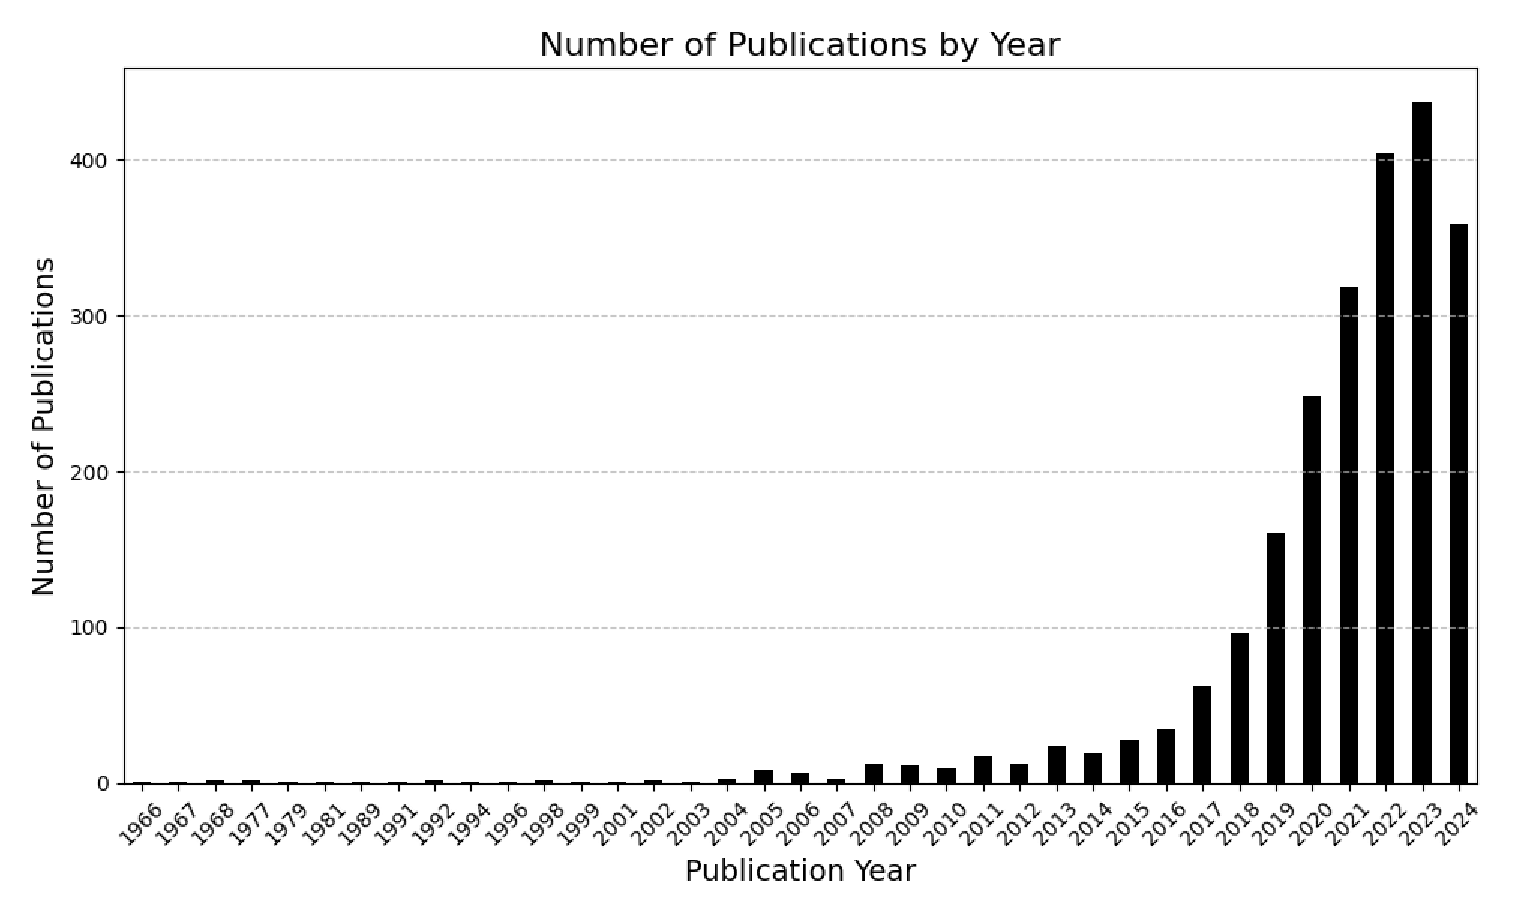
\includegraphics[scale=0.8]{pics/no_publications_year.eps}
		\caption{Distribution of publications across years}\label{fig:fig1}
	\end{figure}
	
	Figures \ref{fig:fig2} show the top 20 authors, the top 20 institutes, and the top 20 countries in terms of number of publications. Considering the authors, we note how the 0.03\% of all authors in our cohort (20 out of 7723) cover over 2.9\% of the total publications, suggesting a skewed distriution of publications across authors. When looking at the top insititutes, we see they cover over 21\% of the total publications (see Table \ref{tab:resdescinst}), while the top 5 countries cover up to 50\% of total publications (see Table \ref{tab:resdesccountry}). Looking deeper into the top insitute, one can notice how many of those Universityies have strong historical bindings with the sea. Consider, as examples, the Dalian Maritime University, the Shangai Maritime Univerity, and the Delft Technical University. Similarly, looking at the most rapresentative countries one can see they all have strong maritime industry and economy.
	
	\begin{figure}[htbp]
		\centering
		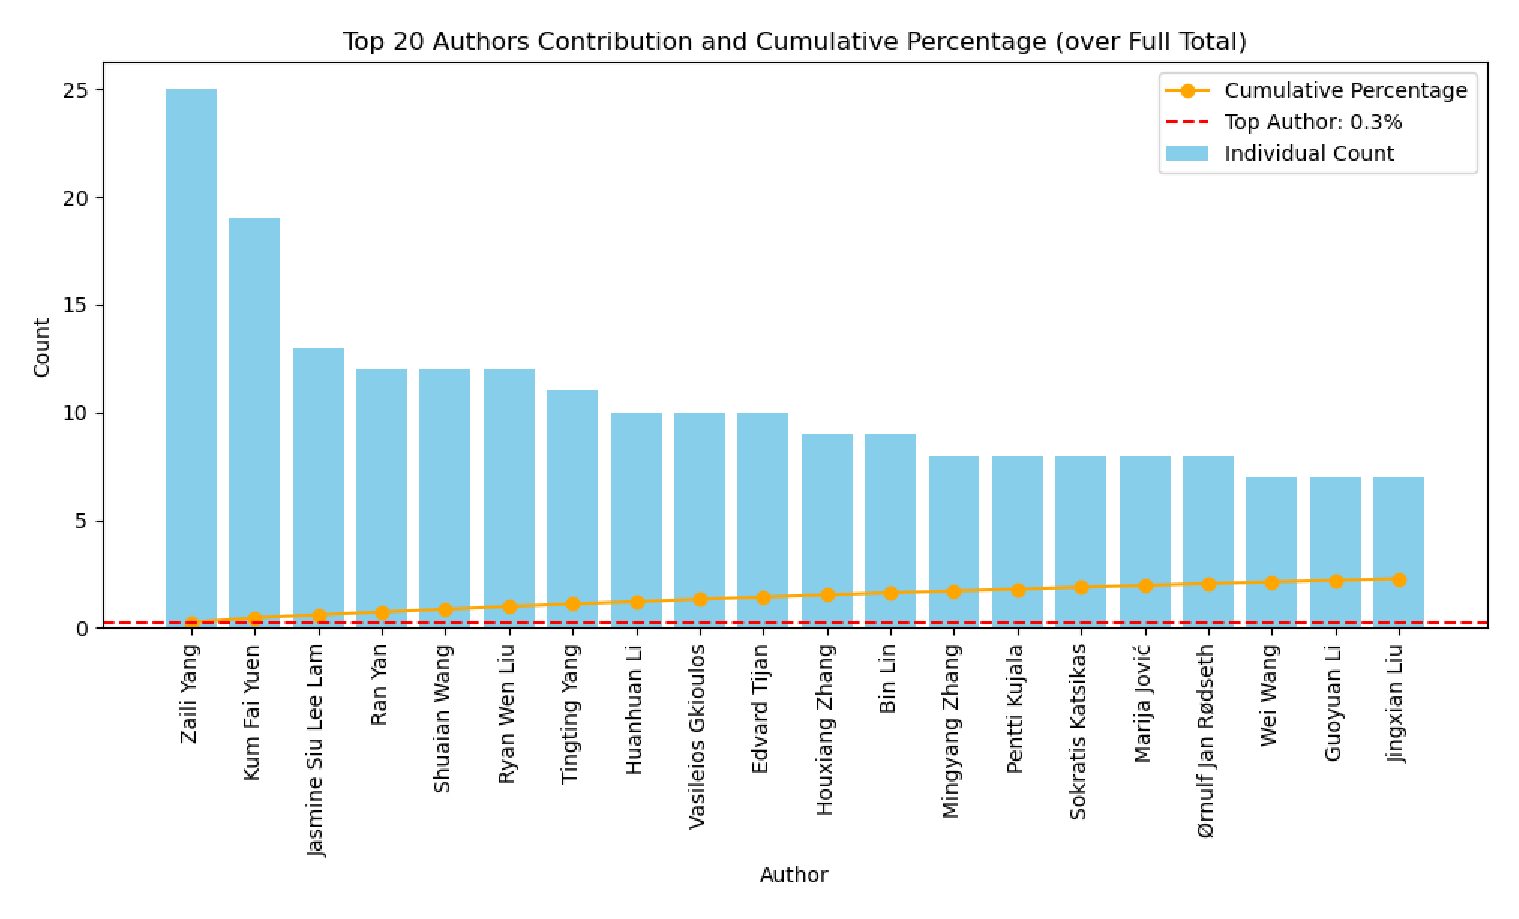
\includegraphics[scale=0.8]{pics/leading_authors.eps}
		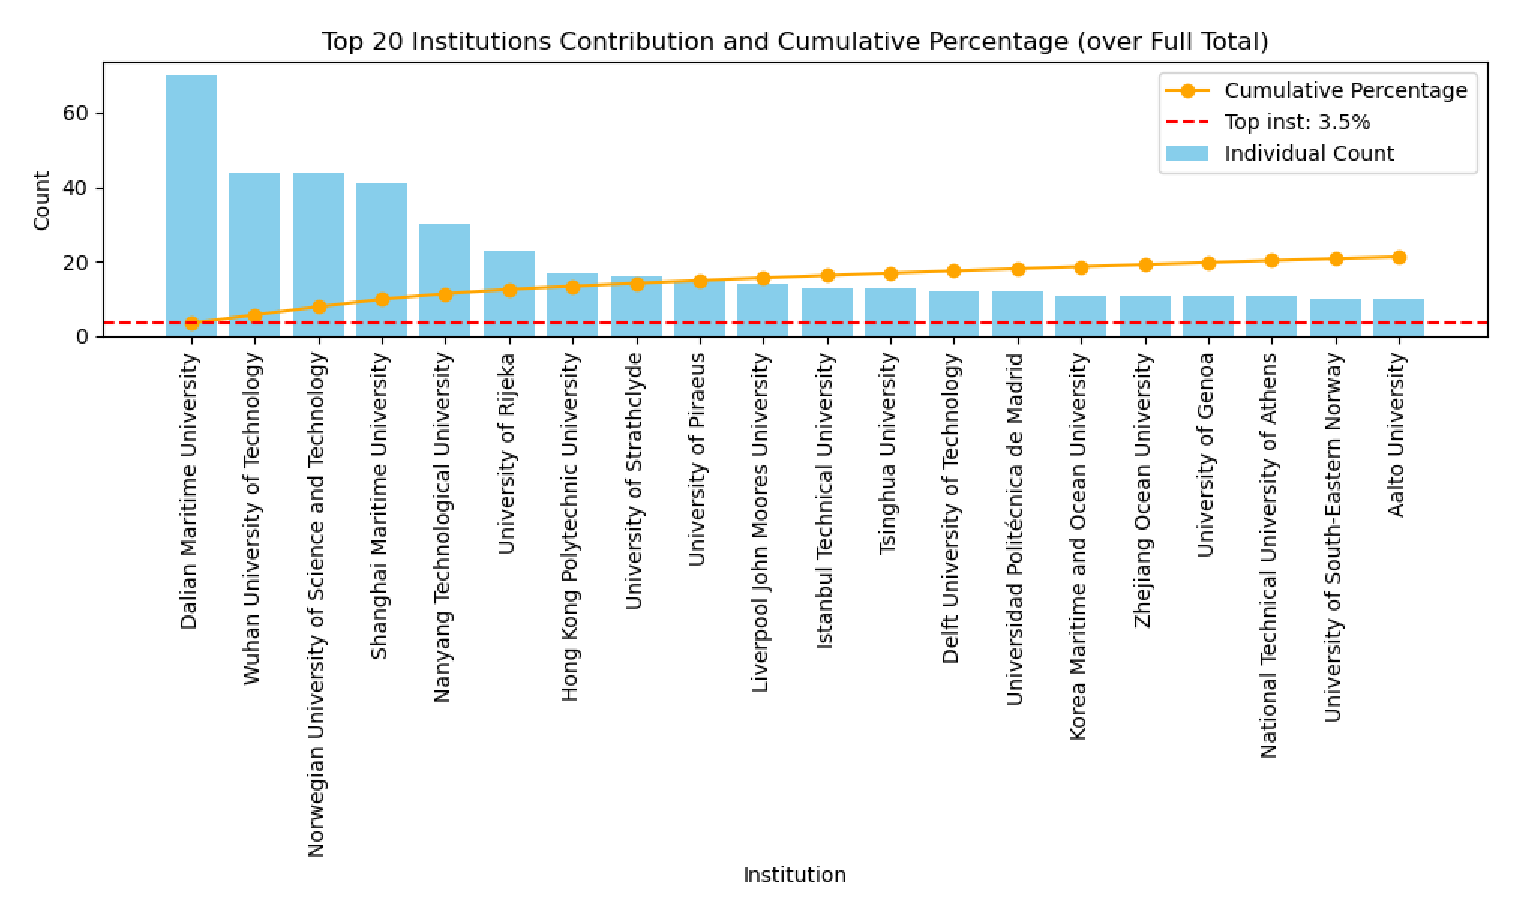
\includegraphics[scale=0.8]{pics/leading_institutions.eps}
		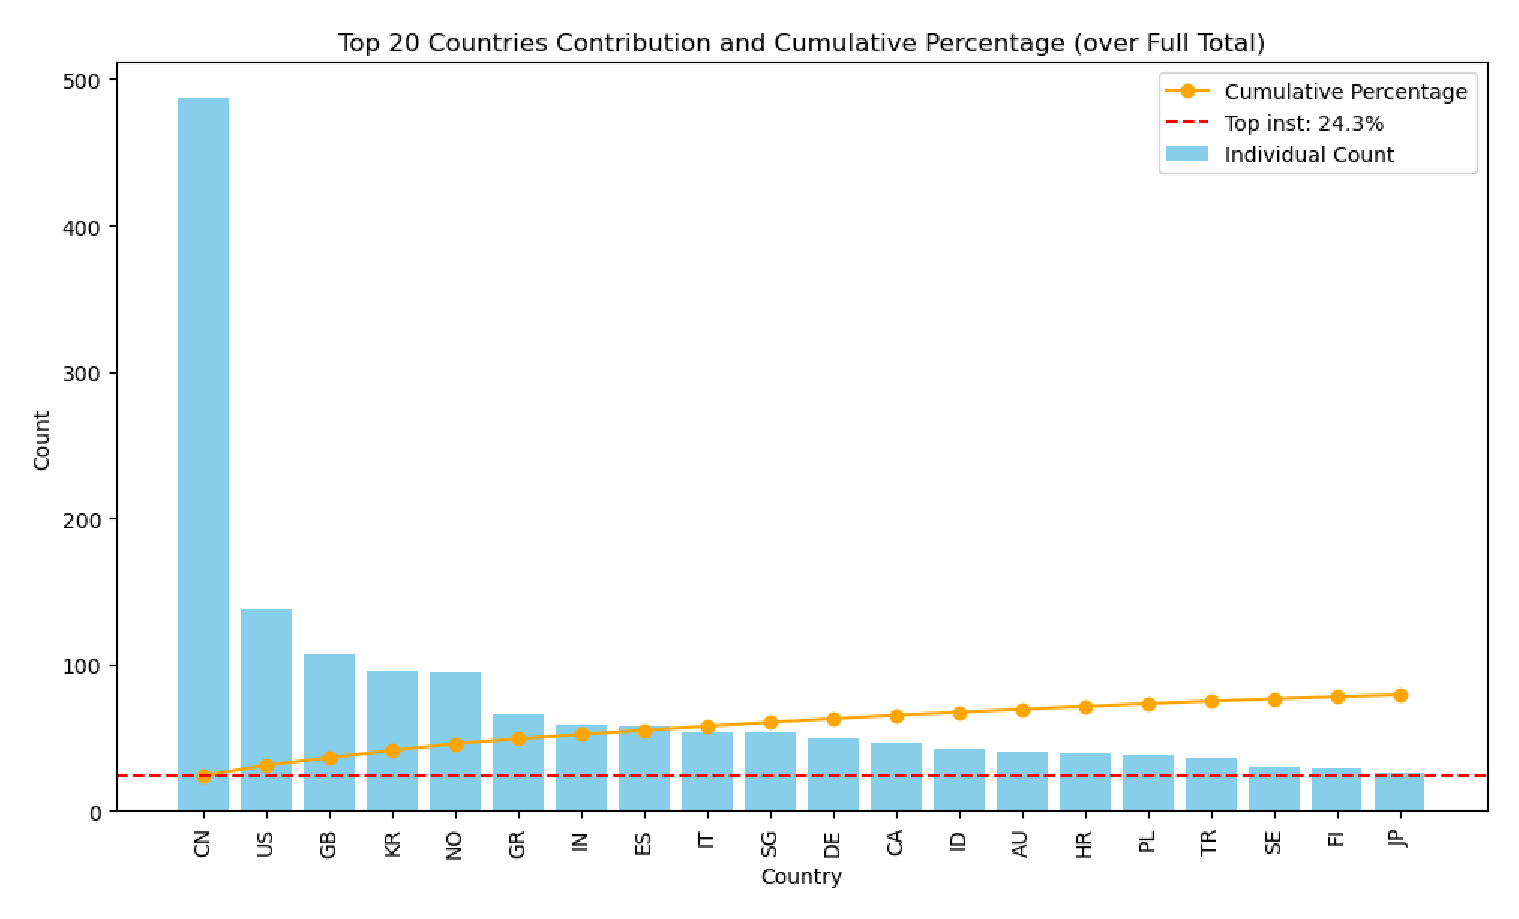
\includegraphics[scale=0.8]{pics/leading_countries.eps}
		\caption{Top 20 leading authors (\textit{top}), institutions (\textit{middle}), and countries (\textit{bottom})}\label{fig:fig2}
	\end{figure}
	
	\begin{table}[h]
		\centering
		\caption{Distribution of publications across institutions.}
		\begin{tabular}{r c c c}
			\hline
			Institution & No. of publications & Cumulative \% & \% Of total \\
			\hline
			Dalian Maritime University & 70 & 3.48 & 3.48\\
			Wuhan University of Technology & 44 & 5.67 & 2.19\\
			Norwegian University of Science and Technology & 44 & 7.86 & 2.19\\
			Shanghai Maritime University & 41 & 9.90 & 2.04\\
			Nanyang Technological University & 30 & 11.39 & 1.50\\
			University of Rijeka & 23 & 12.53 & 1.14\\
			Hong Kong Polytechnic University & 17 & 13.38 & 0.85\\
			University of Strathclyde & 16 & 14.17 & 0.80\\
			University of Piraeus & 15 & 14.92 & 0.75\\
			Liverpool John Moores University & 14 & 15.61 & 0.70\\
			Istanbul Technical University & 13 & 16.26 & 0.65\\
			Tsinghua University & 13 & 16.91 & 0.65\\
			Delft University of Technology & 12 & 17.50 & 0.60\\
			Universidad Politécnica de Madrid & 12 & 18.10 & 0.60\\
			Korea Maritime and Ocean University & 11 & 18.65 & 0.55\\
			Zhejiang Ocean University & 11 & 19.19 & 0.55\\
			University of Genoa & 11 & 19.74 & 0.55\\
			National Technical University of Athens & 11 & 20.29 & 0.55\\
			University of South-Eastern Norway & 10 & 20.79 & 0.50\\
			Aalto University & 10 & 21.28 & 0.50\\
			\hline
		\end{tabular}
		\label{tab:resdescinst}
	\end{table}

	\begin{table}[h]
		\centering
		\caption{Distribution of publications across countries.}
		\begin{tabular}{r c c c}
			\hline
			Country ISO & No. of publications & Cumulative \% & \% Of total \\
			\hline
			CN & 487 & 24.29 & 24.29\\
			US & 138 & 31.17 & 6.88\\
			GB & 107 & 36.51 & 5.34\\
			KR & 96 & 41.30 & 4.79\\
			NO & 95 & 46.03 & 4.73\\
			GR & 66 & 49.33 & 3.29\\
			IN & 59 & 52.27 & 2.94\\
			ES & 58 & 55.16 & 2.89\\
			IT & 54 & 57.86 & 2.69\\
			SG & 54 & 60.55 & 2.69\\
			DE & 50 & 63.04 & 2.49\\
			CA & 47 & 65.39 & 2.34\\
			ID & 42 & 67.48 & 2.09\\
			AU & 40 & 69.48 & 2.00\\
			HR & 39 & 71.42 & 1.95\\
			PL & 38 & 73.32 & 1.90\\
			TR & 36 & 75.11 & 1.80\\
			SE & 30 & 76.61 & 1.50\\
			FI & 29 & 78.05 & 1.45\\
			JP & 26 & 79.35 & 1.30\\
			\hline
		\end{tabular}
		\label{tab:resdesccountry}
	\end{table}

	\subsection{Co-authorship network analysis}
	The degree distribution of the co-authorship network seems to follow a power-law curve (see Fig. \ref{fig:fig3}. However, several distributions may present similar curves. To establish which is the best fitting model we run statistical tests. We run statistical tests, calculating the log-likelihood and p-value between different pairs. The power-law distribution was significantly more accurate fit than the exponential one (p \textless 0.01). However, the comparison between power-law and truncated power-law distributions, as well as the one between power-law and log-normal distributions, did not lead to significantly different results (p=0.32 and p=0.39 respectively). The results confirm the heavy-tail characteristic of the degree distribution (which holds true for both log-normal and power-law), but without further indicate the possible nature of such heavy tail \citep{mitzenmacher2004brief,higaki2020co,liu2021structural,smith2021explaining}.
	
	\begin{figure}[htbp]
		\centering
		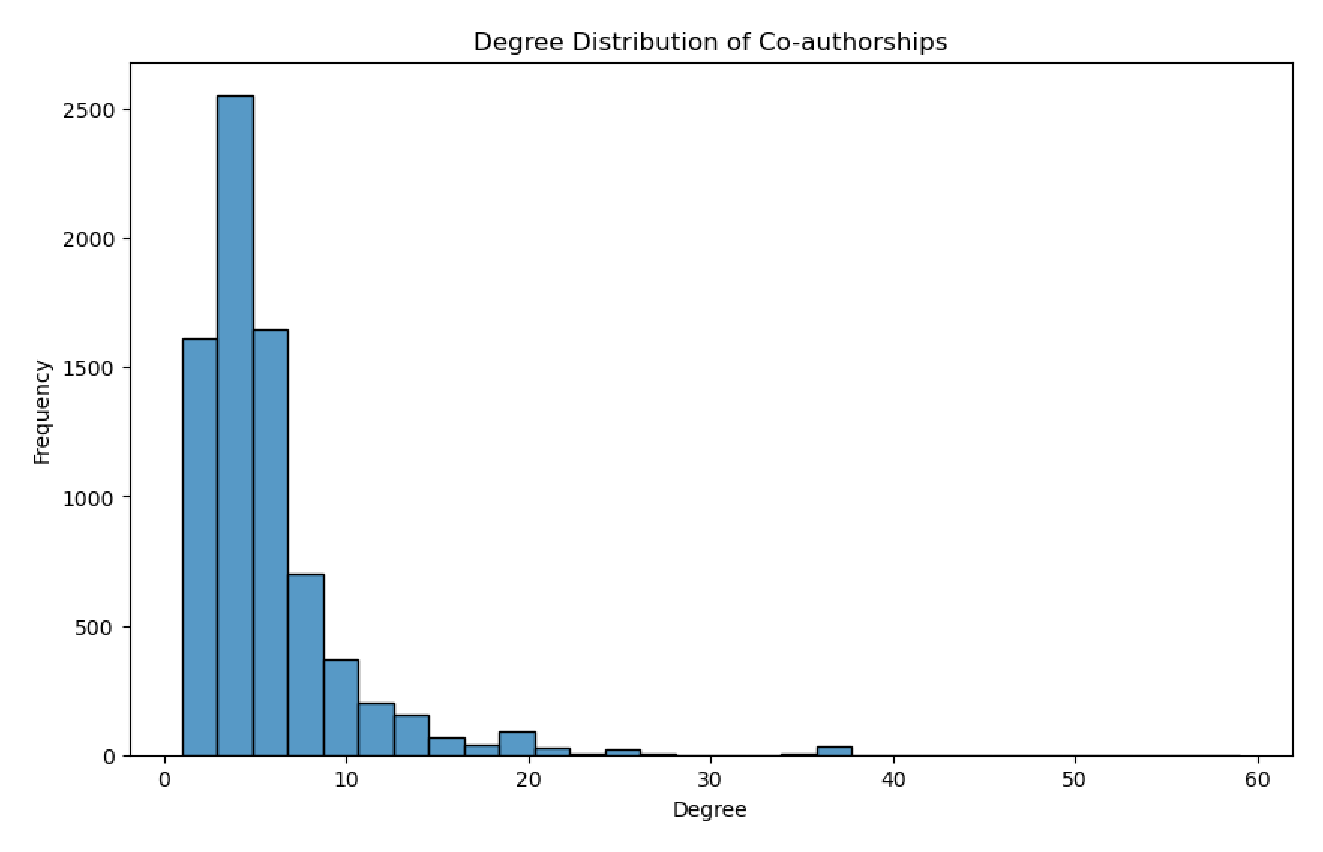
\includegraphics[scale=0.8]{pics/coauthorship_degree_distribution.eps}
		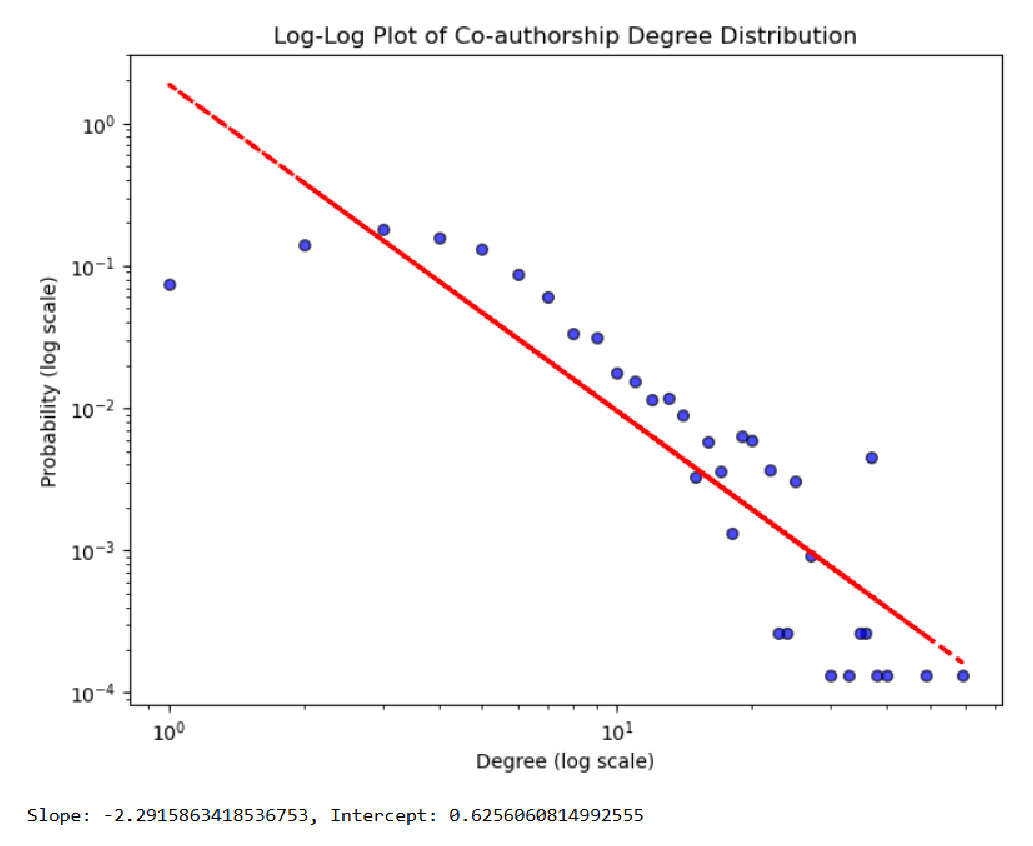
\includegraphics[scale=0.8]{pics/coauthorship_degree_distribution_loglog_chart.eps}
		\caption{Co-authorship degree distribution (\textit{top}), and corresponding log-log chart (\textit{bottom})}\label{fig:fig3}
	\end{figure}
	
	As a second step in our co-authorship network analysis, we identified the largest component of the network (made of 2753 authors), and identified its main communities, using the Louvain algorithm \citep{blondel2008fast}. We identified 28 communities (see Fig. \ref{fig:fig4}), and map on them the distribution of institutions and countries linked to the authors. Results highlight a high level of international collaborations within each community, as well as a high level of national collaborations (within the same country). This can be seen in Figure \ref{fig:fig5}, where we show the number of different countries and institutions per community. Furthermore, our network analysis does not show and closed cluster of collaborations. Communities are all well inter-connected, suggesting that the niche nature of this field (i.e., digital transformation in shipping) leads global actors to collaborate extensively in advancing research. In Figure [XXX] and Figure [XXX] we show the chord charts for both country and institution mapping on the co-authorship communities.
	
	\begin{figure}[htbp]
		\centering
		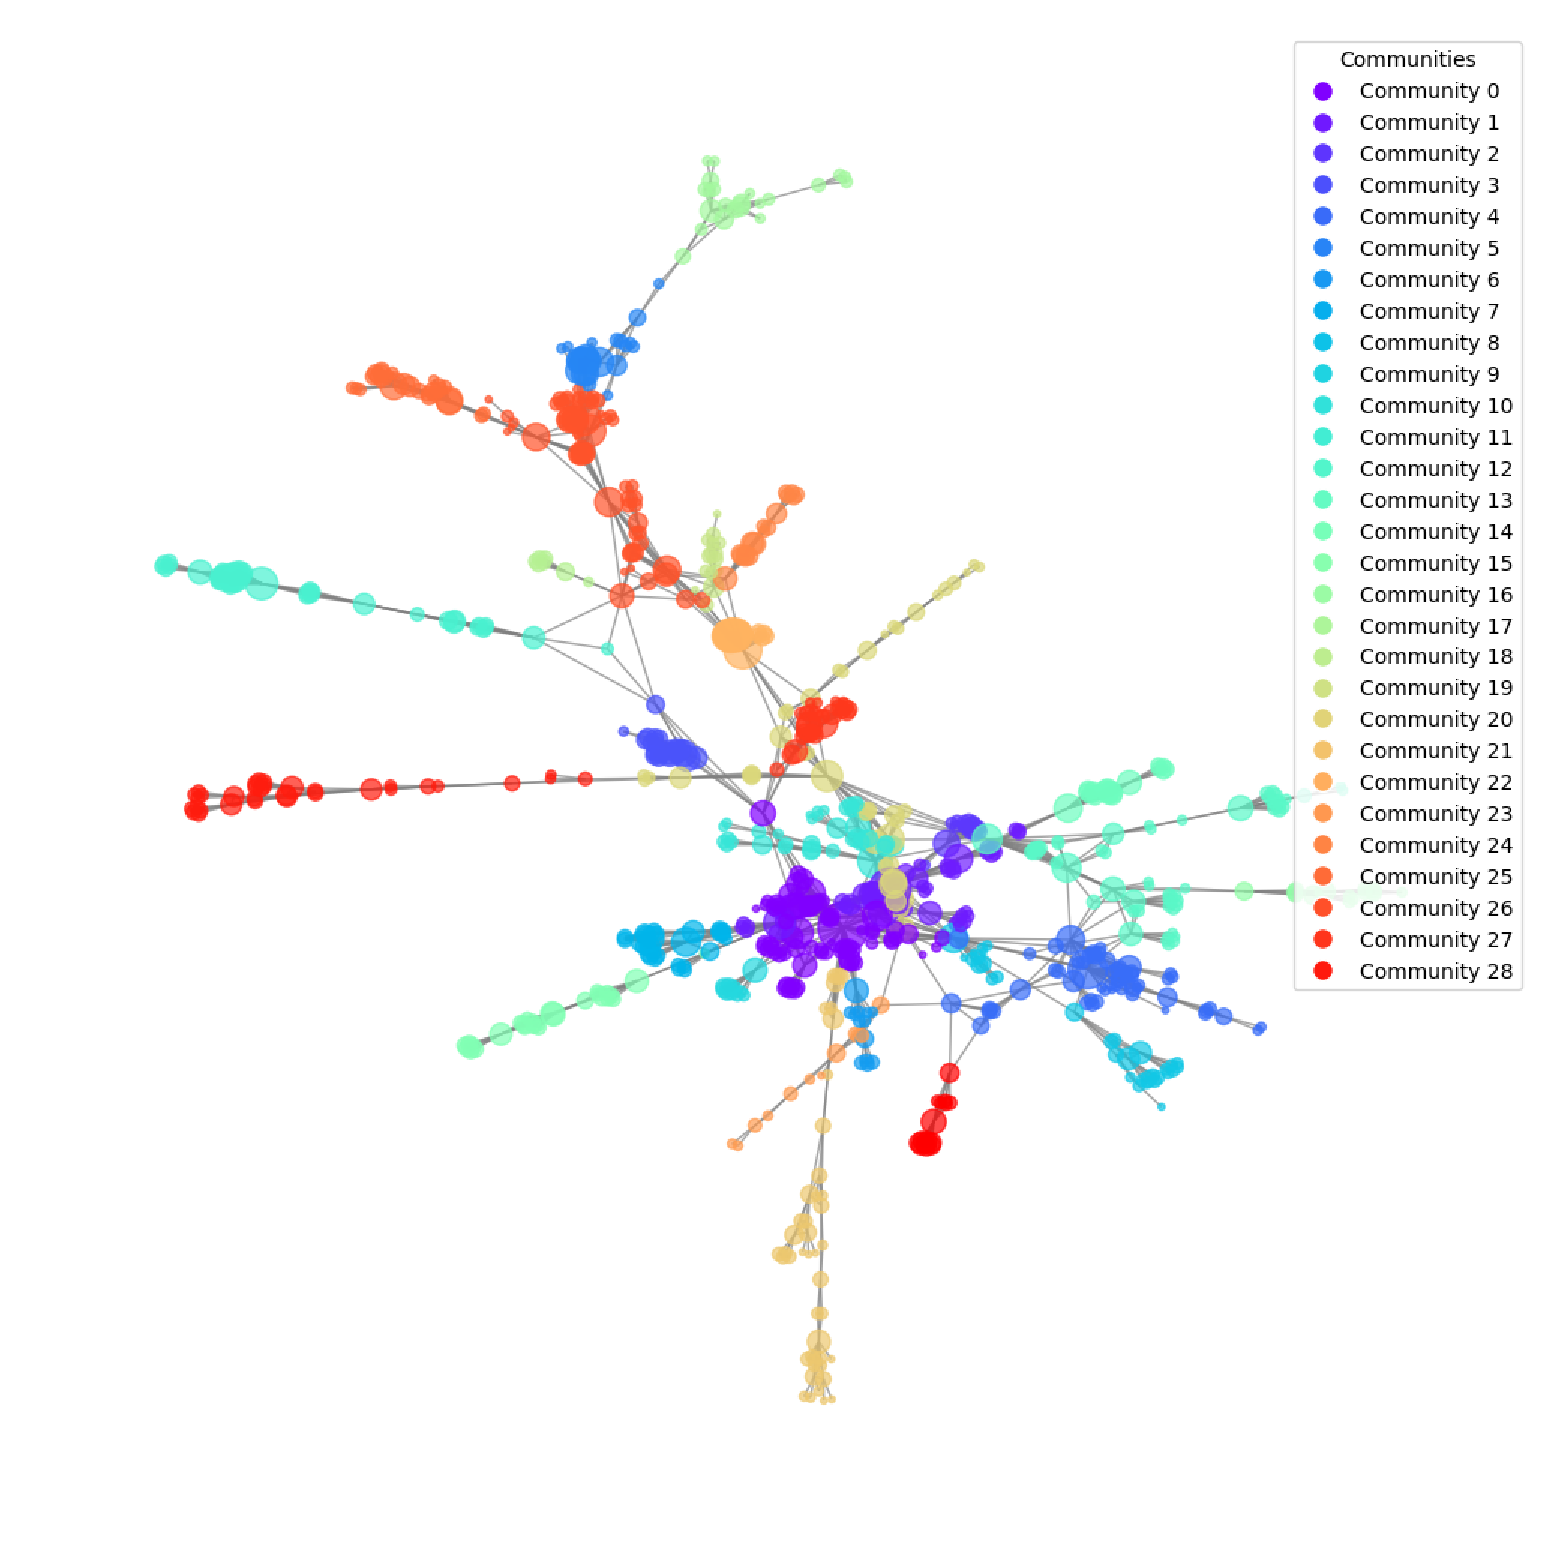
\includegraphics[scale=0.8]{pics/co-authorship_communities.eps}
		\caption{Co-authorship network with communities}\label{fig:fig4}
	\end{figure}
	
	\begin{figure}[htbp]
		\centering
		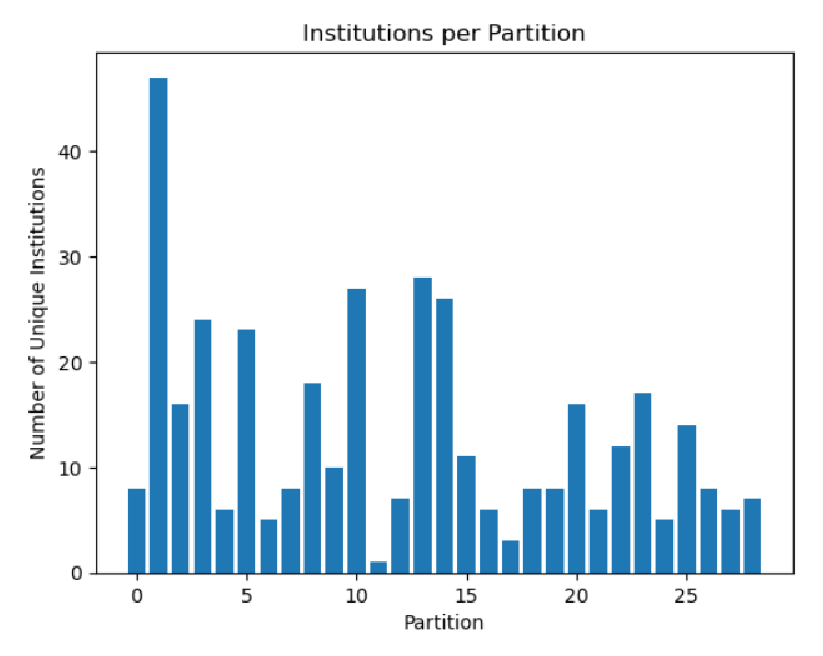
\includegraphics[scale=0.8]{pics/coauthorship_inst_per_partition.eps}
		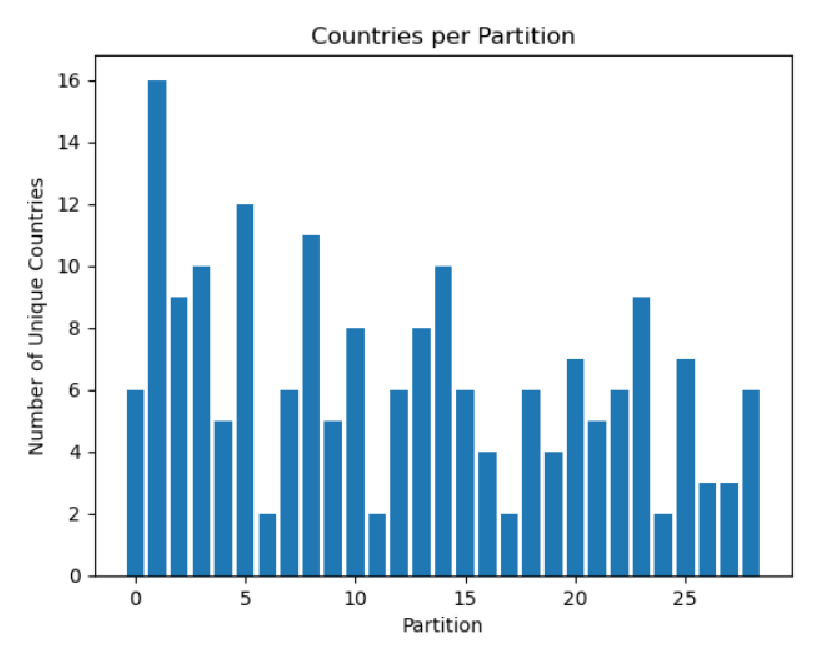
\includegraphics[scale=0.8]{pics/coauthorship_country_per_partition.eps}
		\caption{Co-authorship distribution of insitutions (\textit{top}) and countries (\textit{bottom}) across partitions}\label{fig:fig5}
	\end{figure}

	\begin{figure}[htbp]
		\centering
		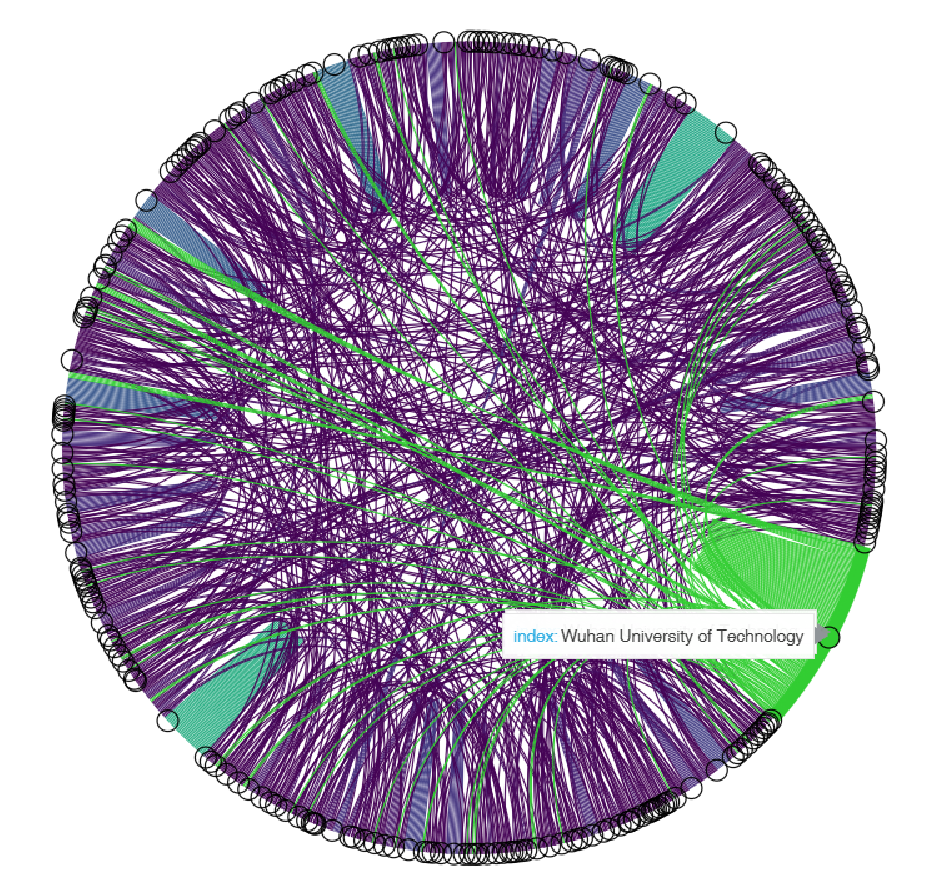
\includegraphics[scale=0.8]{pics/coauthorship_inst_chord_1.eps}
		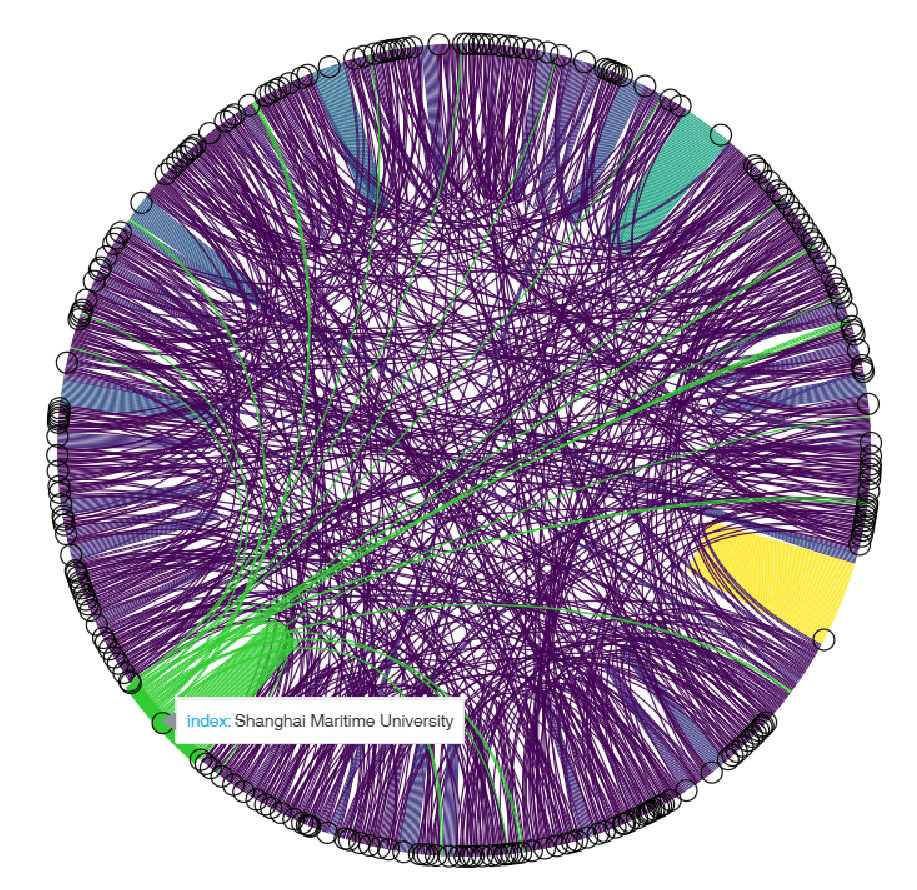
\includegraphics[scale=0.8]{pics/coauthorship_inst_chord_2.eps}
		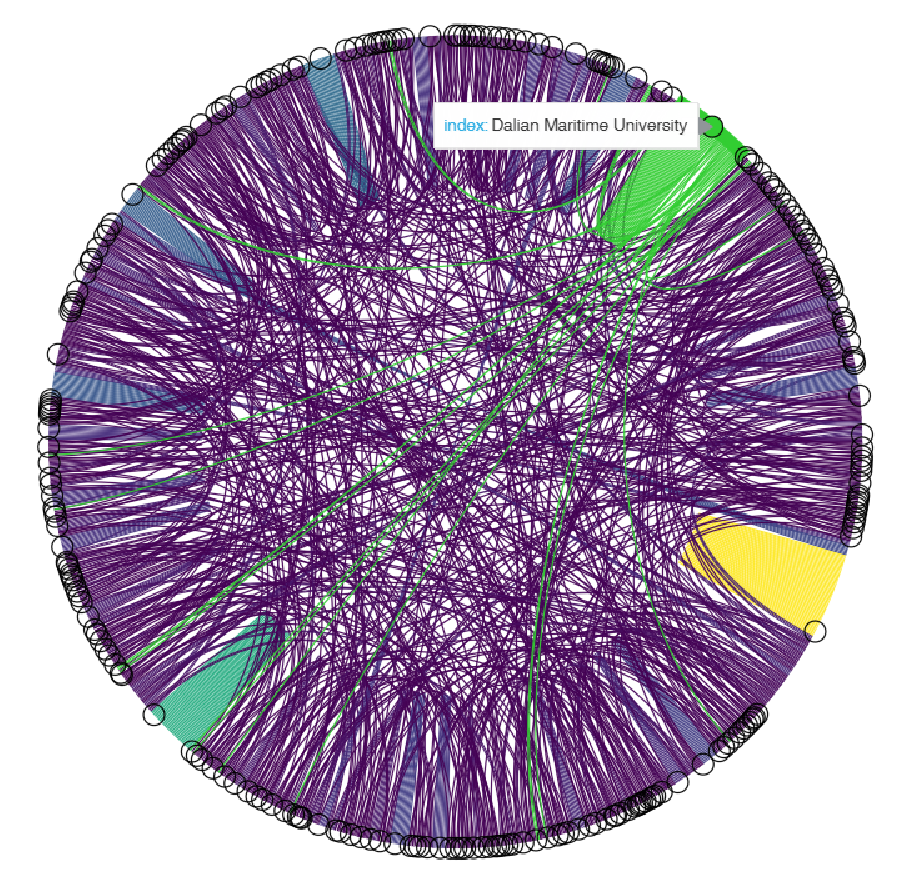
\includegraphics[scale=0.8]{pics/coauthorship_inst_chord_3.eps}
		\caption{Chord diagrams for insitution mapping on co-authorship communities. The three diagrams show three relevant clusters: (\textit{top}) XXX, (\textit{middle}) XXX, and (\textit{bottom}) XXX}\label{fig:fig6}
	\end{figure}

	\begin{figure}[htbp]
		\centering
		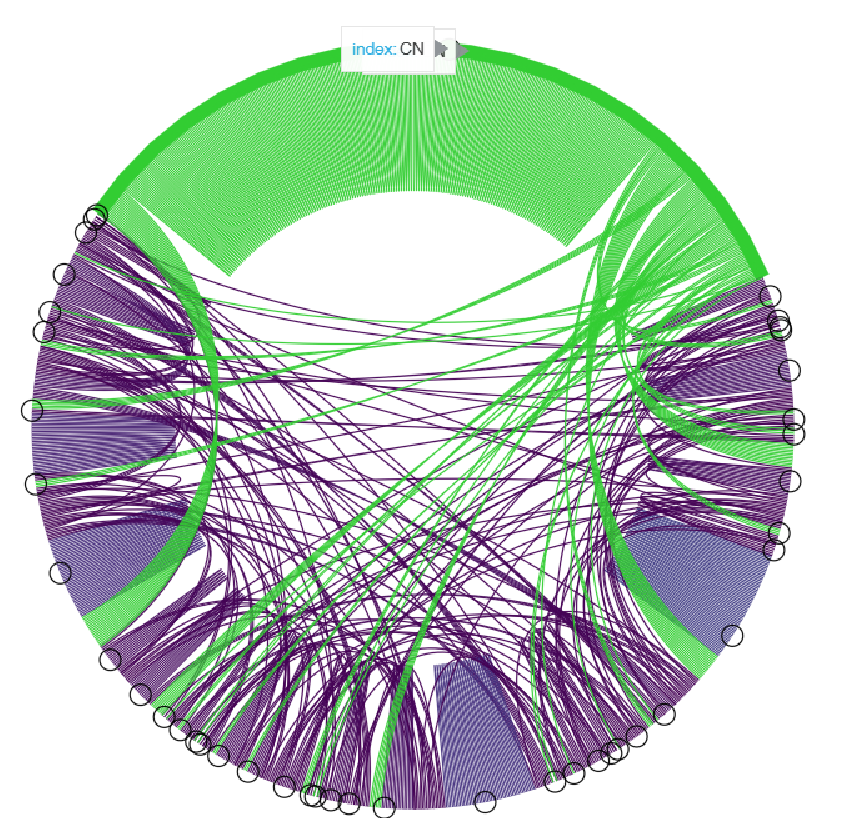
\includegraphics[scale=0.8]{pics/coauthorship_country_chord_1.eps}
		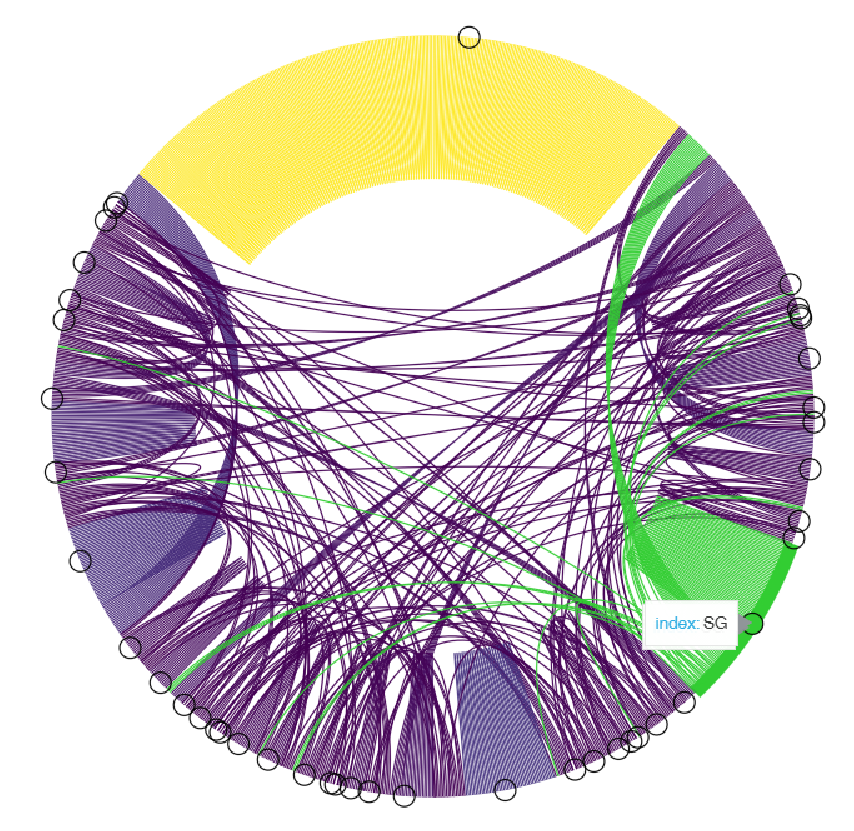
\includegraphics[scale=0.8]{pics/coauthorship_country_chord_2.eps}
		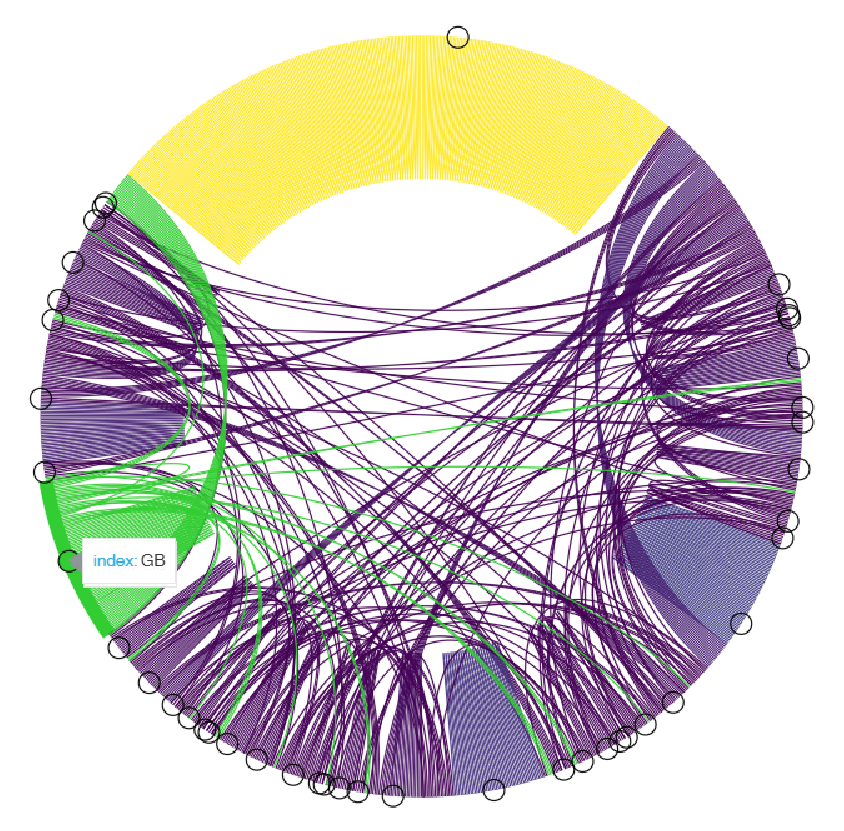
\includegraphics[scale=0.8]{pics/coauthorship_country_chord_3.eps}
		\caption{Chord diagrams for countries mapping on co-authorship communities. The three diagrams show three relevant clusters:(\textit{top}) XXX, (\textit{middle}), and (\textit{bottom}) XXX}\label{fig:fig7}
	\end{figure}
	
	Lastly, we evaluated the small-world properties of the co-authorship network. To do so, we calculated both clustering coefficient and average path length, and compare them with equivalent random networks. Our results show a higher clustering coefficient (0.83 vs 0.007) and a higher average path (7.1 vs. 3.9). In a proper small-world topology, one would expect high clustering coefficient and small average path. Our results, instead, suggest that communities are strongly locally organized, but somehow lack efficiency in cross community communication.
	
	\subsection{Co-citation network analysis}
	The co-citation network was analyzed for its largest connected component (made of 1298 articles). The results on the degree distribution are similar to those we obtained for the co-authorship network. More specifically, the statistical comparison between degree distribution excluded an exponential distribution (p \textless 0.05), and did not favor a power-law distribution against log-normal or truncated power-law distribution (p=0.06 and p=0.9 respectively). Figure \ref{fig:fig8} shows the degree distribution.
	
	\begin{figure}[htbp]
		\centering
		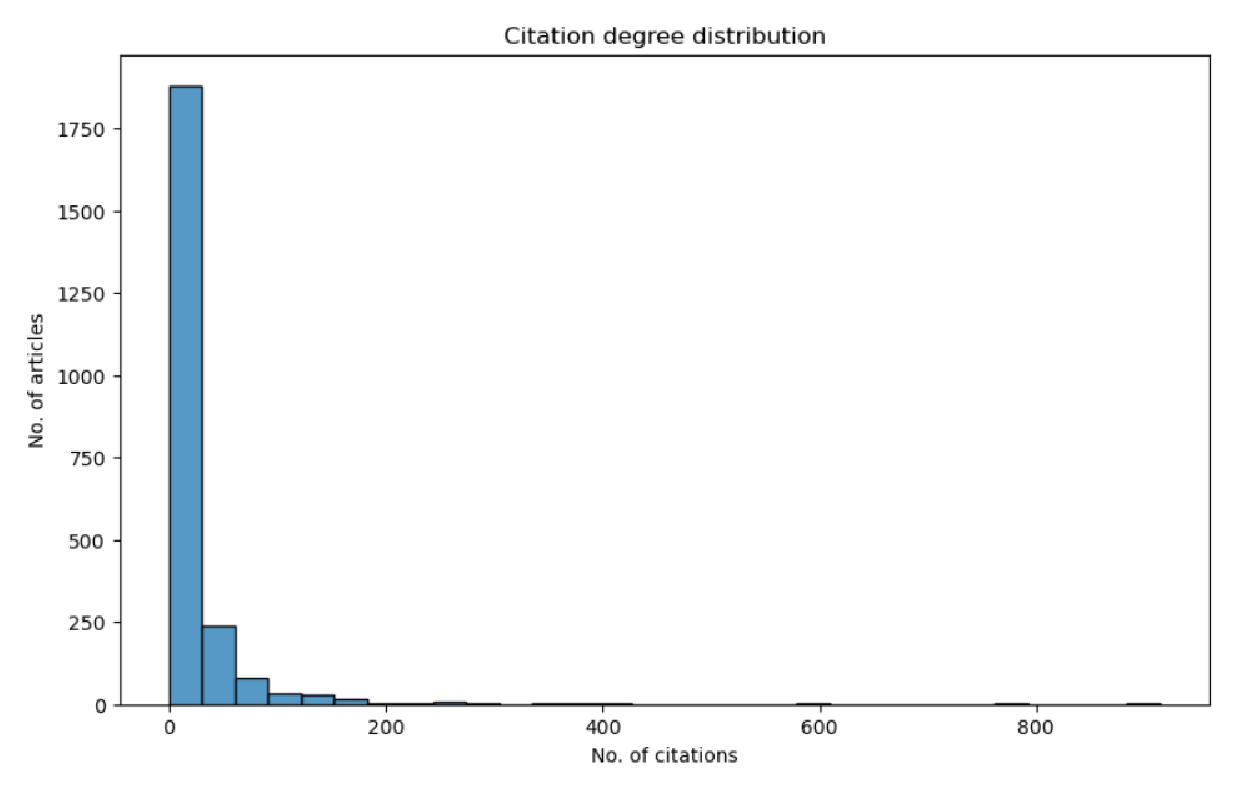
\includegraphics[scale=0.8]{pics/citation_degree_distribution.eps}
		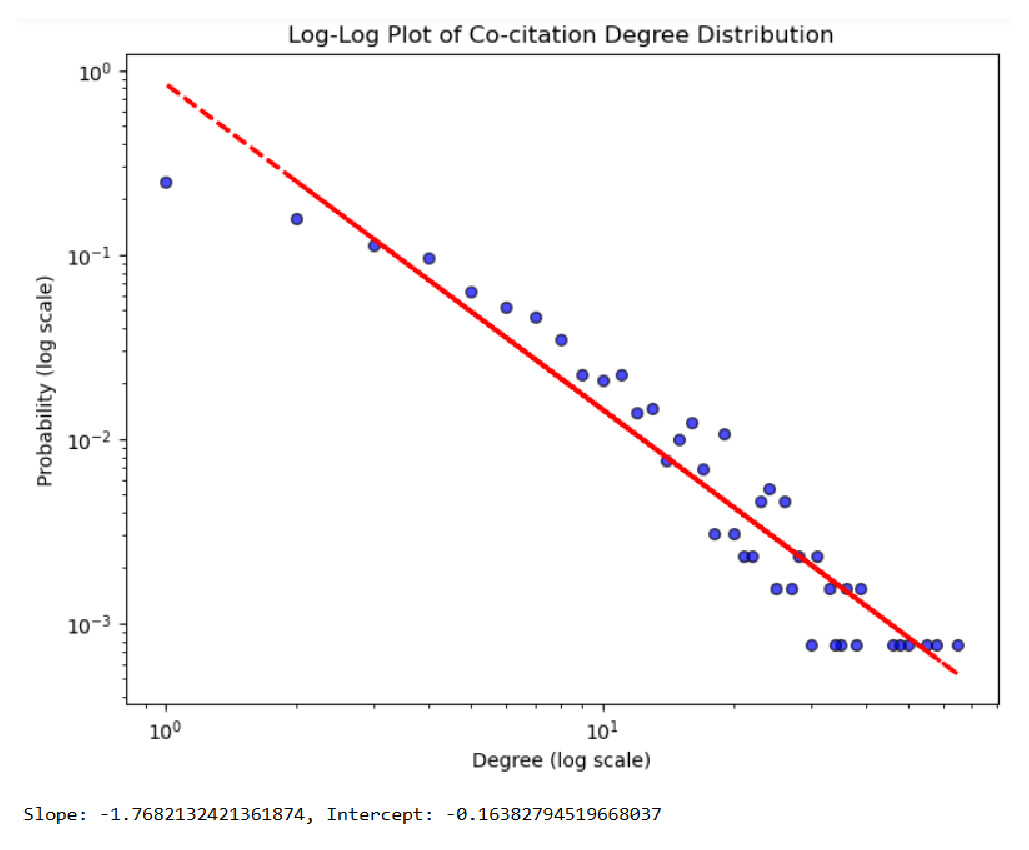
\includegraphics[scale=0.8]{pics/loglog_citation_degree_distribution.eps}
		\caption{Co-citation degree distribution and log-log chart} \label{fig:fig8}
	\end{figure}
	
	Using the degree distribution, we identified the most influential articles (i.e. top 10 articles with the highest number of co-citation). Table \ref{tab:citationtoppapers} shows such influential works. One can see that amongh the most influential works we find SLRs and bibliometric studies, supporting the relevance of such publicaitons within the industry.
	
	\begin{table}[h]
		\centering
		\caption{Top 10 influential papers based on citations.}
		\begin{tabular}{l l c}
			\hline
			DOI & Title & Publication Year\\
			\hline
			https://doi.org/10.1080/03088839.2020.1788731 & Big data and artificial intelligence in the maritime industry: a bibliometric review and future research directions & 2020\\
			https://doi.org/10.3390/jmse12060919 & Comprehensive Analysis of Maritime Cybersecurity Landscape Based on the NIST CSF v2. 0 & 2024\\
			https://doi.org/10.1016/j.tre.2019.09.020 & Maritime shipping digitalization: Blockchain-based technology applications, future improvements, and intention to use & 2019\\
			https://doi.org/10.1080/01441647.2019.1649315 & How big data enriches maritime research–a critical review of Automatic Identification System (AIS) data applications & 2019\\
			https://doi.org/10.3390/app14145994 & Harnessing AI for sustainable shipping and green ports: Challenges and opportunities & 2024\\
			https://doi.org/10.1016/j.ijcip.2022.100571 & Developments and research directions in maritime cybersecurity: A systematic literature review and bibliometric analysis & 2022\\
			https://doi.org/10.1109/tits.2019.2908191 & Traffic pattern mining and forecasting technologies in maritime traffic service networks: A comprehensive survey & 2019\\
			https://doi.org/10.3390/s19040926 & Toward Digitalization of Maritime Transport? & 2019\\
			https://doi.org/10.3390/info13010022 & Cyber security in the maritime industry: A systematic survey of recent advances and future trends & 2022\\
			https://doi.org/10.3390/jmse10040486 & Digitalization in maritime transport and seaports: bibliometric, content and thematic analysis & 2022\\
			\hline
		\end{tabular}
		\label{tab:citationtoppapers}
	\end{table}
	
	Next, we created a sub-graph considering only the 20\% most cited articles (257 nodes). We identified the communities using the Louvain algorithm and perform a topic analysis on the titles of the articles per community. Table \ref{tab:citationthemes} reports the main topics for each of the 7 communities we identified, while Figure \ref{fig:fig9} show the color-mapped communities.
	
	\begin{figure}[htbp]
		\centering
		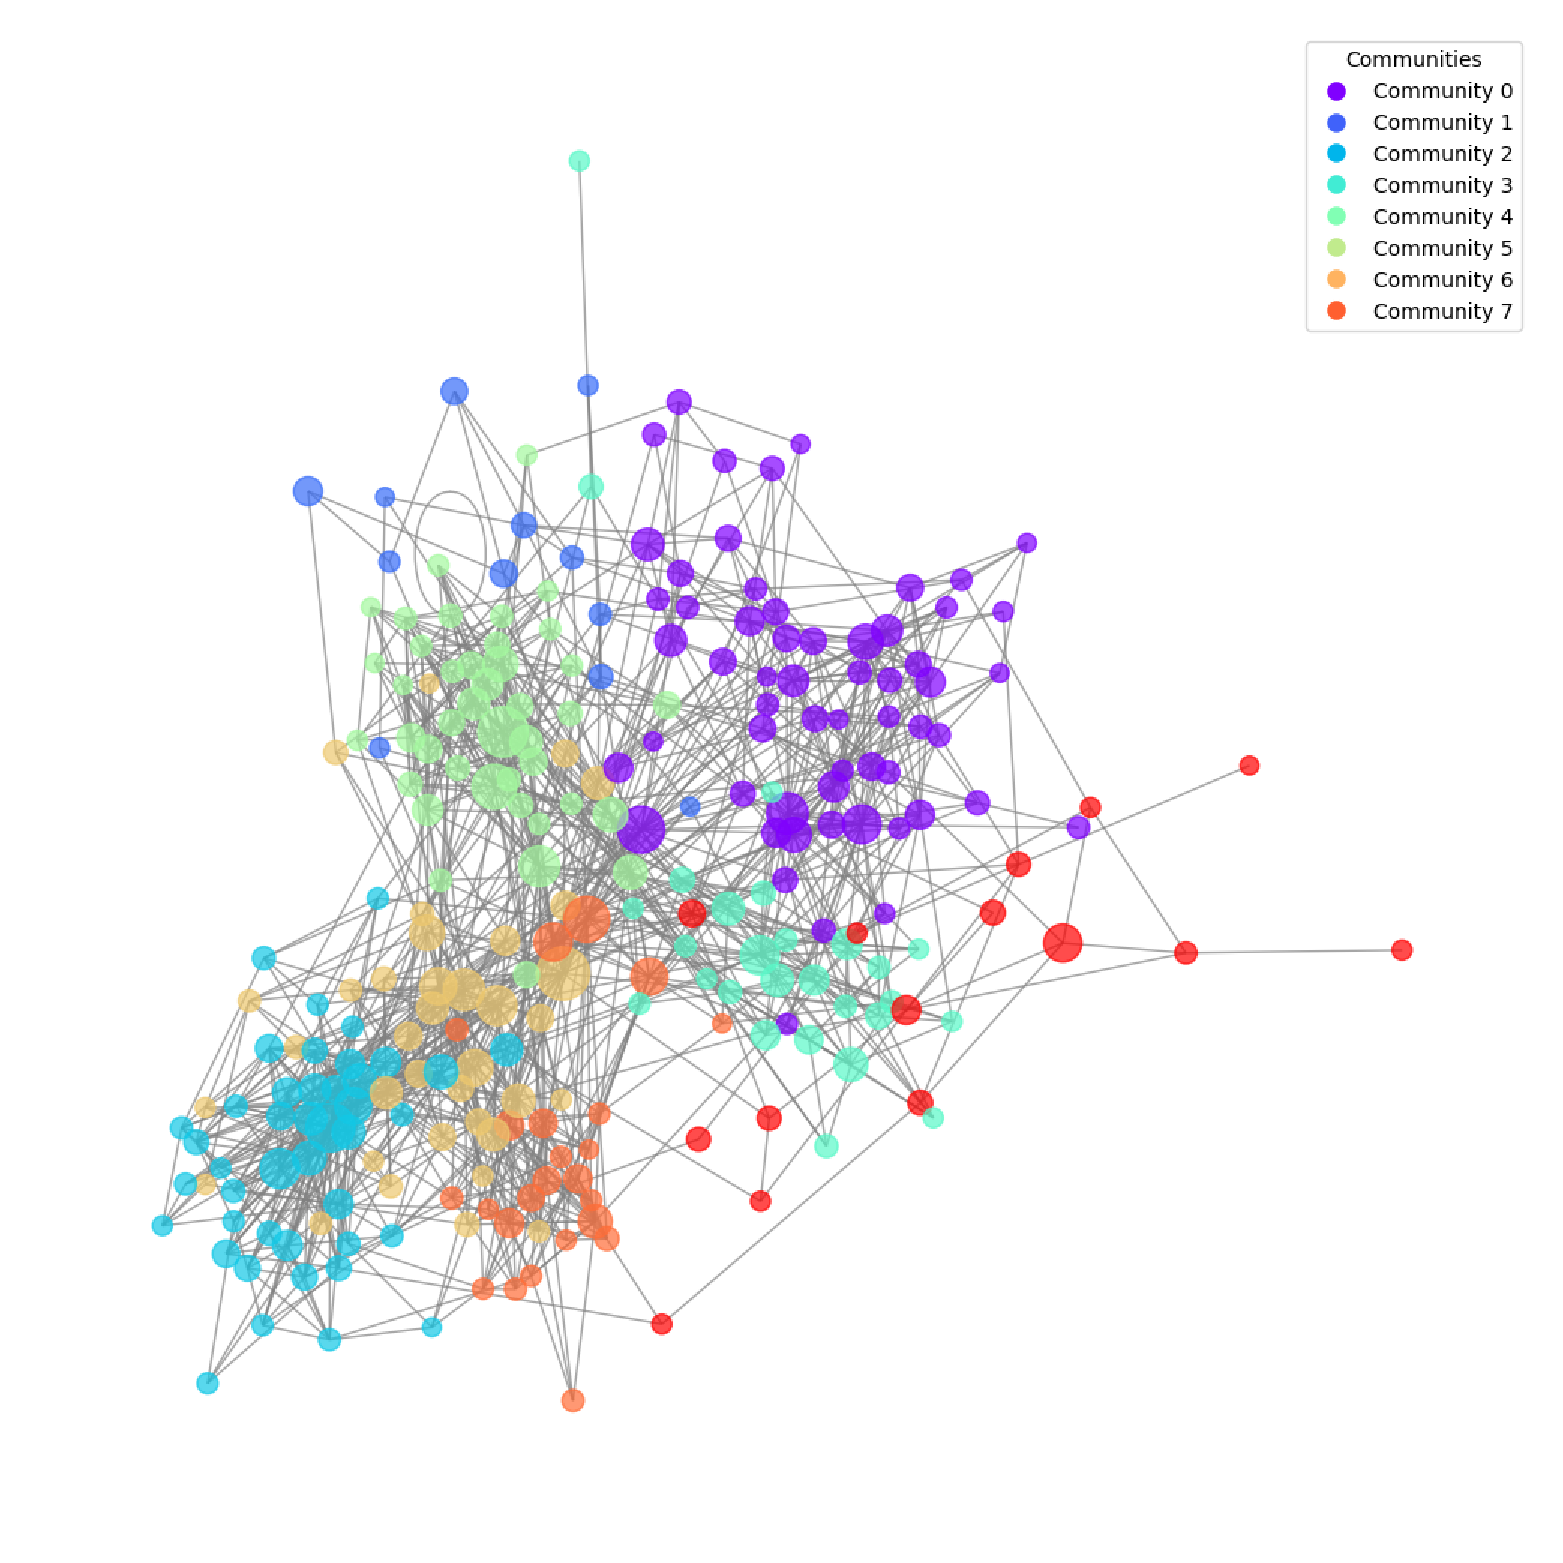
\includegraphics[scale=0.8]{pics/cocitation_communiities.eps}
		\caption{Co-citation network with communities}\label{fig:fig9}
	\end{figure}
	
	\begin{table}[h]
		\centering
		\caption{Community-based topic analysis}
		\begin{tabular}{l l c}
			\hline
			Community & Main theme \\
			\hline
			1 & Optimization and prediction of fuel consumption, energy efficiency, and environmental impact in the maritime industry, with a focus on machine learning, big data, and modeling techniques.\\
			2 & Maritime safety, risk management, and the application of machine learning techniques to predict, analyze, and mitigate accidents and hazards in maritime operations. \\
			3 & Machine learning, artificial intelligence, and big data applications in the maritime domain.\\
			4 & Integration of Internet of Things (IoT), mobile edge computing, communication networks, and security within the maritime industry, with a particular focus on autonomous ships, data offloading, latency minimization, and communication technologies for maritime transportation systems.\\
			5 & Digital transformation and technological advancements within the maritime sector, particularly in relation to maritime logistics, container shipping, port operations, and the broader shipping supply chain.\\
			6 & Development and optimization of smart ports, focusing on the integration of Industry 4.0 technologies.\\
			7 & Maritime cybersecurity, with an emphasis on cyber risks associated with the digital transformation of the maritime industry, particularly as it pertains to the rise of autonomous vessels, smart shipping technologies, and the IoT-enabled maritime environment.\\
			8 & Adoption and application of blockchain technology in the maritime industry, specifically in areas like shipping, supply chains, and port management.\\
			\hline
		\end{tabular}
		\label{tab:citationthemes}
	\end{table}
	
	Finally, we adopted several centrality measures to identify the most relevant articles. More specifically, we identified the 5 top articles for five different centrality measures: degree centrality, betweenness centrality, closeness centrality, eigenvector centrality, and page rank. We union the results and identified 10 relevant articles for further analysis. We then looked more in details to the theme covered in these articles to extrapolate relevant research areas the field. Results are shown in Table \ref{tab:citationcentrality}.
	
	\begin{table}[h]
		\centering
		\caption{Centrality-based topic analysis.}
		\begin{tabular}{l l c}
			\hline
			OpenAlex ID & Top 5 in N centrality measures & Main topic \\
			\hline
			W3041382323	& 5 & Big data and artificial intelligence\\
			W4400493457	& 4 & Artificial intelligence, sustainable shipping, and green ports\\
			W2964482263	& 4 & Big data\\
			W2978644098	& 3 & Blockchains\\
			W4386245296	& 2 & Data and IoT\\
			W4225993858	& 2 & Digitalization\\
			W4399283331	& 2 & Cybersecurity\\
			W3090216936	& 1 & Blockchain conceptual framework\\
			W4205557186	& 1 & Cybersecurity\\
			W3213918042	& 1 & Blockchain\\
			\hline
		\end{tabular}
		\label{tab:citationcentrality}
	\end{table}
		
	\subsection{Thematic analysis}
	For the thematic analysis, we considered all titles from the 2290 articles. After having pre-processed, tokenized, and vectorized all titles, we used clustering methods to identify the best number of clusters for the vectors. More specifically, we used the Calinski-Harabasz index and the Davies-Bouldin index. The curves are shown in Figure \ref{fig:fig10}. All indexes pointed to 8 ideal clusters. For each cluster, we calculated the centroid and then selected the 10 closest vectors (i.e. articles) to each centroid. Focusing on their titles, we highlighted the main themes for each cluster. Results are shown in Table \ref{tab:thematic}.
	
	\begin{figure}[htbp]
		\centering
		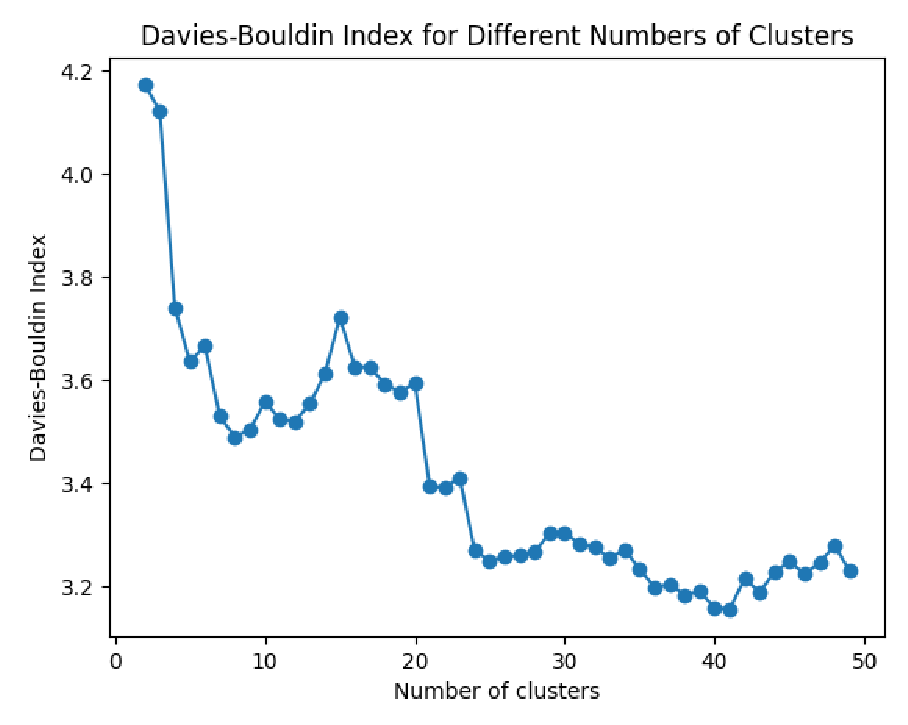
\includegraphics[scale=0.8]{pics/davis_bouldin.eps}
		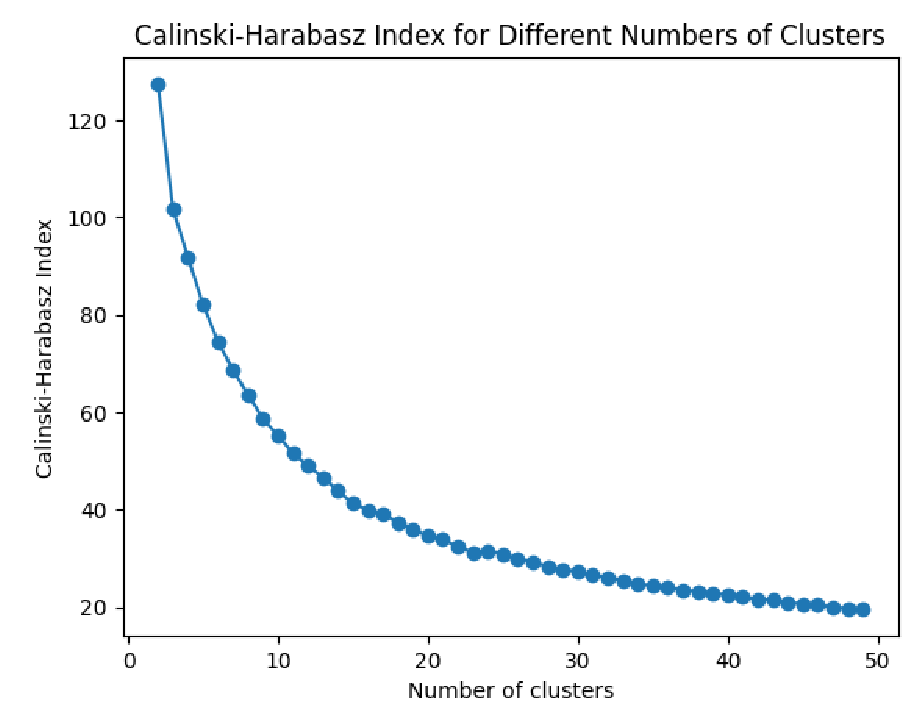
\includegraphics[scale=0.8]{pics/calinski.eps}
		\caption{Davies-Bouldin (\text{top}) and Calinski-Harabasz (\textit{bottom}) indexes.}\label{fig:fig10}
	\end{figure}
	
	\begin{table}[h]
		\centering
		\caption{Results of thematic analysis.}
		\begin{tabular}{l}
			\hline
			\textbf{Topic 1: Advancements in AI and Machine Learning for Maritime Applications}. This topic explores the integration of advanced AI techniques in the maritime sector, focusing on automation, situational awareness, and safety. Articles discuss multi-scale object detection models for autonomous ship navigation and the use of UAVs for data collection and surveillance. Research includes adaptive data fusion for vessel trajectory prediction and machine learning frameworks for maritime anomaly detection, such as sensor-based monitoring systems and beamforming for communication. The use of explainable AI frameworks for anomaly detection and multi-task learning for vessel draft reading emphasizes intelligent decision-making and safety in maritime operations.\\			
			\textbf{Topic 2: Spatial and Environmental Analysis in Maritime and Inland Waters}. This topic focuses on the intersection of spatial data analysis, environmental monitoring, and maritime operations. Studies include remote sensing for water monitoring, spatial planning for offshore wind energy, and machine learning applications in greenhouse gas emission modeling. Research spans risk assessment for maritime transportation, air quality forecasting, and maritime accidents influenced by environmental factors like sea fog. The use of geographically weighted regression and big data for analyzing maritime transportation reflects a growing trend in environmental and geospatial analytics.\\			
			\textbf{Topic 3: Predictive Modeling and Risk Assessment in Maritime Operations.} This topic delves into predictive models and analytics for enhancing safety and efficiency in maritime activities. Research highlights fuel consumption modeling, arrival time prediction, and the trust dynamics in supervising autonomous ships. Big data and machine learning approaches are employed for evaluating ship grounding risks, collision probability, and traffic safety. Several articles focus on in-depth traffic and economic analyses, emphasizing data-driven decision-making in maritime operations.\\			
			\textbf{Topic 4: Data-Driven Optimization in Maritime Engineering and Traffic Management.} This topic addresses the use of data-driven and AI approaches in ship design, traffic prediction, and environmental forecasting. Articles discuss applications of machine learning, such as predicting wave heights, optimizing ship design under uncertainty, and evaluating traffic in multi-port systems. Risk assessment of sea lanes and carbon emission forecasting highlight the push toward sustainable and efficient maritime engineering solutions.\\			
			\textbf{Topic 5: Blockchain and Edge Computing in Maritime Operations.} This topic investigates the application of blockchain and edge computing technologies in maritime logistics and communication. Research focuses on blockchain-enabled vulnerability detection, data integrity, and privacy-preserving data sharing. Articles highlight innovative use cases, such as smart contracts for shipping efficiency, decentralized anomaly detection systems, and reliable communication frameworks. These technologies aim to enhance maritime transport security, efficiency, and data transparency.\\			
			\textbf{Topic 6: Innovations and Reviews in Autonomous and Smart Shipping.} This topic reviews the state of autonomous and smart shipping technologies, exploring their implications for design, safety, and logistics. Studies analyze machine learning in sustainable ship design, the current status of MASS (Maritime Autonomous Surface Ships) technologies, and digital twins for shipboard systems. Articles also examine functional suitability assessments of smart contracts and the bibliometric review of risk and reliability in autonomous systems. These discussions highlight the transformative potential of digitalization in maritime logistics.\\			
			\textbf{Topic 7: Digital Transformation and Sustainability in Maritime Logistics.} This topic focuses on the digitalization of maritime operations and its impact on sustainability and efficiency. Articles explore blockchain’s role in digital transformation, automation's impact on gender parity, and renewable energy adoption in seaports. The use of deep learning for vessel trajectory prediction and intelligent supervision through network analysis underscores the push for smart maritime systems. The integration of data spaces and IoT technologies highlights innovative solutions for managing logistics and maritime operations sustainably.\\			
			\textbf{Topic 8: Maritime Industry’s Adaptation to Digital and Sustainable Practices.} This topic explores the maritime industry's response to emerging technologies and sustainability challenges. Articles examine digital transformation strategies, blockchain adoption, and risk management performance in start-ups. Studies analyze sustainability reports and explore environmental risks through a 20-year analysis of maritime accidents. Research emphasizes co-creation in operations management, addressing sustainability goals through technological and organizational innovations.\\
			\hline
		\end{tabular}
		\label{tab:thematic}
	\end{table}
	
	Next, we built words cloud for our articles. In this case, we used both title and abstract words. A first word cloud was built using all words after pre-processing them. The second word cloud was built after remoing shipping related key words. This allowed us to focus on technical key words for the second word cloud. Both word clouds were based on TF-IDF analysis and are shown in Figure \ref{fig:fig11} and Figure \ref{fig:fig12}.
	
	\begin{figure}[htbp]
		\centering
		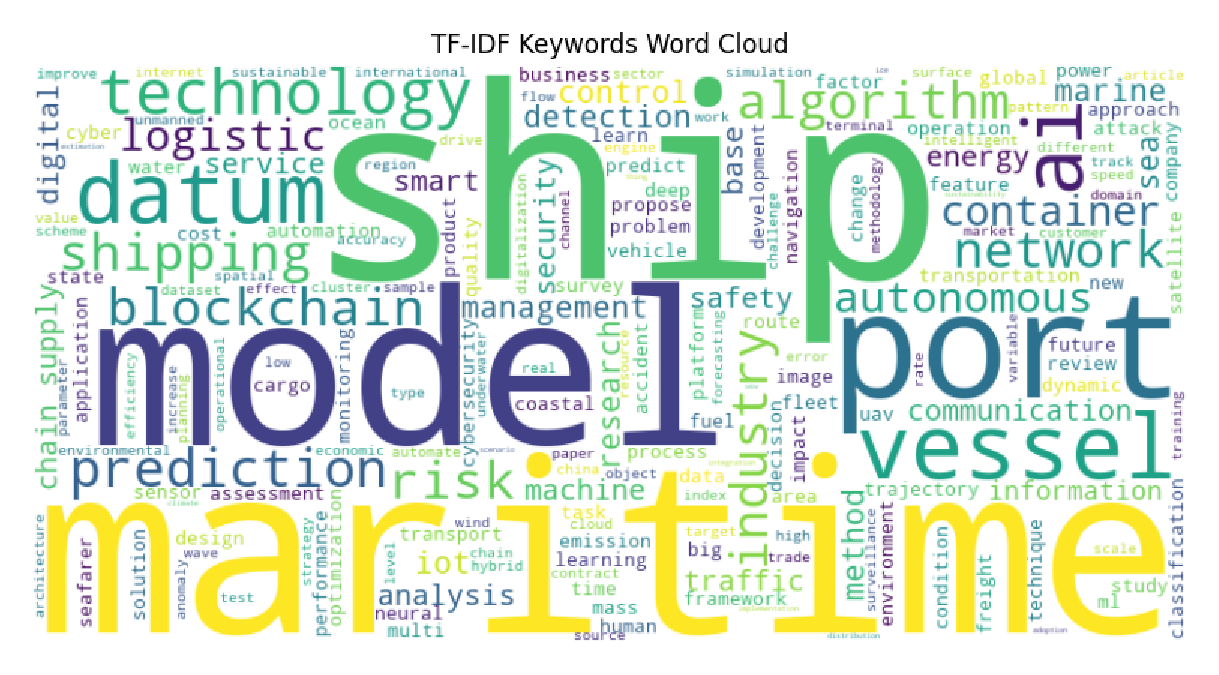
\includegraphics[scale=0.8]{pics/wordcloud_1.eps}
		\caption{Word cloud based on TF-IDF}\label{fig:fig11}
	\end{figure}
	
	\begin{figure}[htbp]
		\centering
		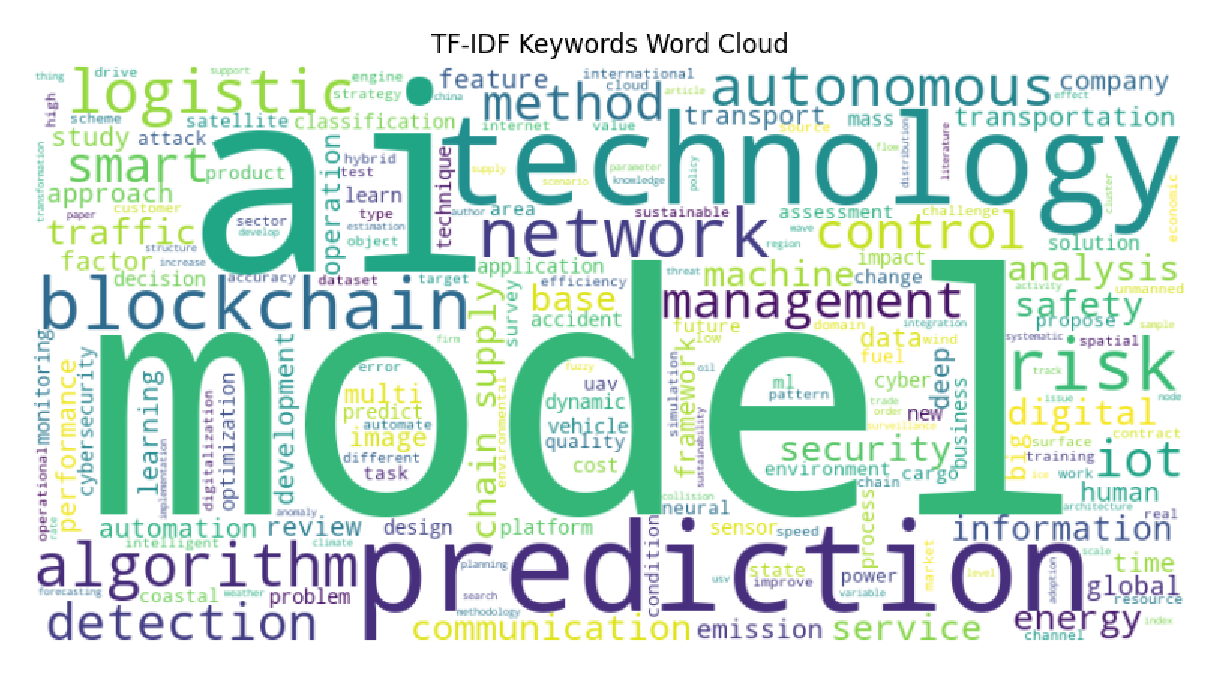
\includegraphics[scale=0.8]{pics/wordcloud_2.eps}
		\caption{Word cloud focused on technological terms}\label{fig:fig12}
	\end{figure}
	
	As a last analysis, we focused on the concept tags reported by OpenAlex for each paper. OpenAlex organized topics in a tree-like structure which is a modification of the one produced by \citep{shen2018web}. Specifically, there are 19 root-level concepts: engineering, computer science, business, economics, philosophy, mathematics, political science, medicine, psychology, environmental science, geology, geography, chemistry, physics, biology, sociology, art, history, and materials science. We have collected the root-level concepts related to the publications in out study and plot the number of corresponding papers over time (see Figure \ref{fig:fig13}).
	
	\begin{figure}[htbp]
		\centering
		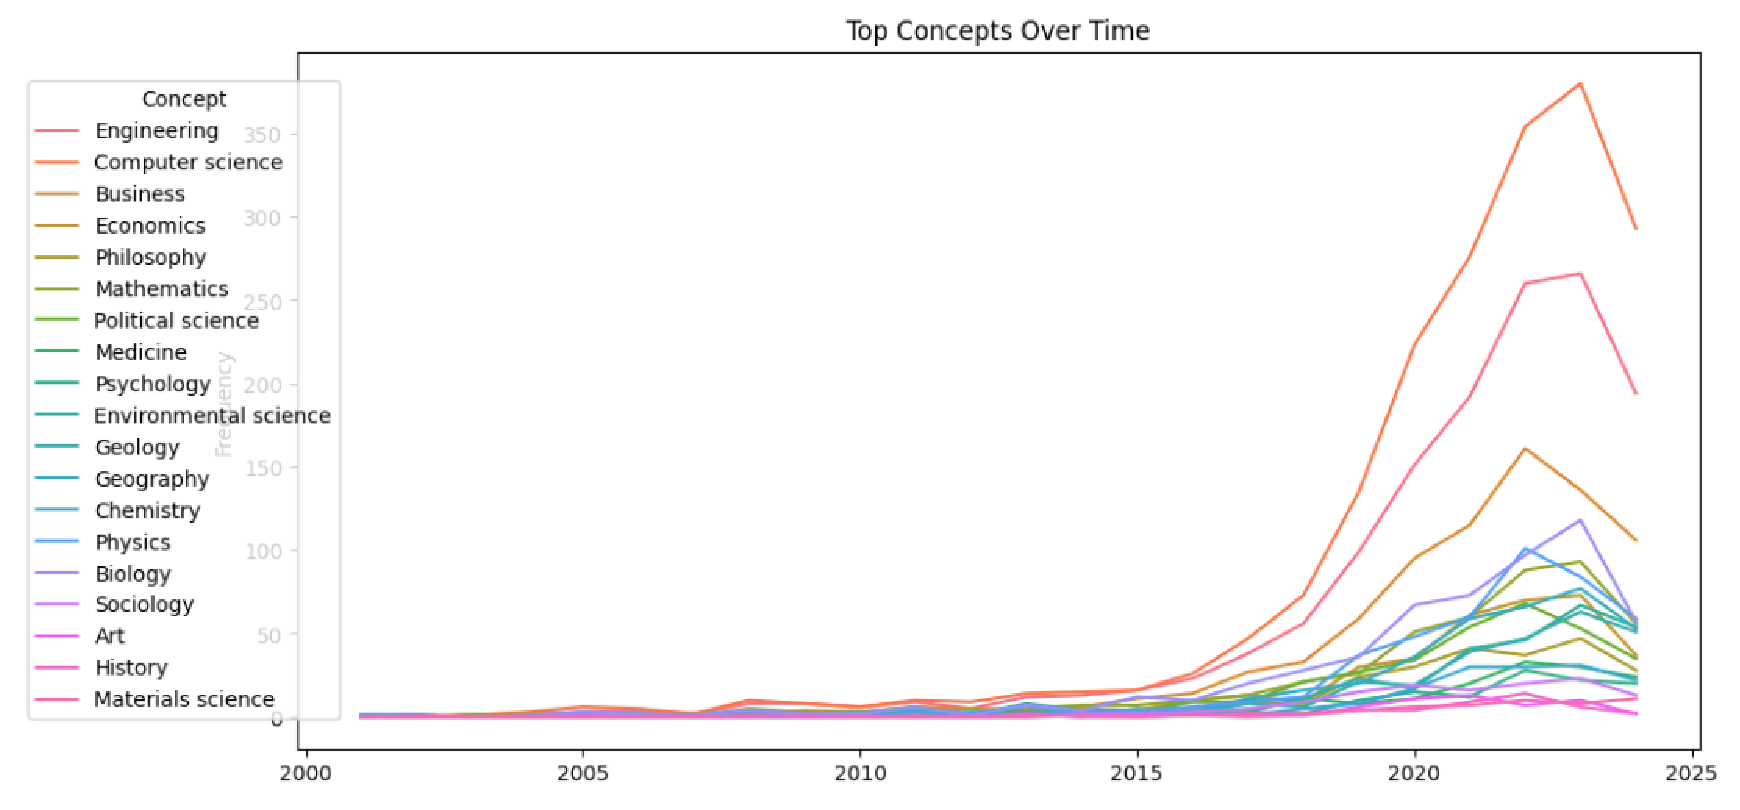
\includegraphics[scale=0.8]{pics/main_concept_trend_toplevel.eps}
		\caption{Top-level OpenAlex concept distribution over time terms}\label{fig:fig13}
	\end{figure}
	
	The predominant top-level concept over time are engineering, computer science, and business. We next focused on the second and third level of concepts of Open-Alex, limiting our search to those having as parents either engineering, computer science, or business. Among those, we selected the 10 most relevant and showed their evolution over time in a heatmap (see Figure \ref{fig:fig14}).
	
	\begin{figure}[htbp]
		\centering
		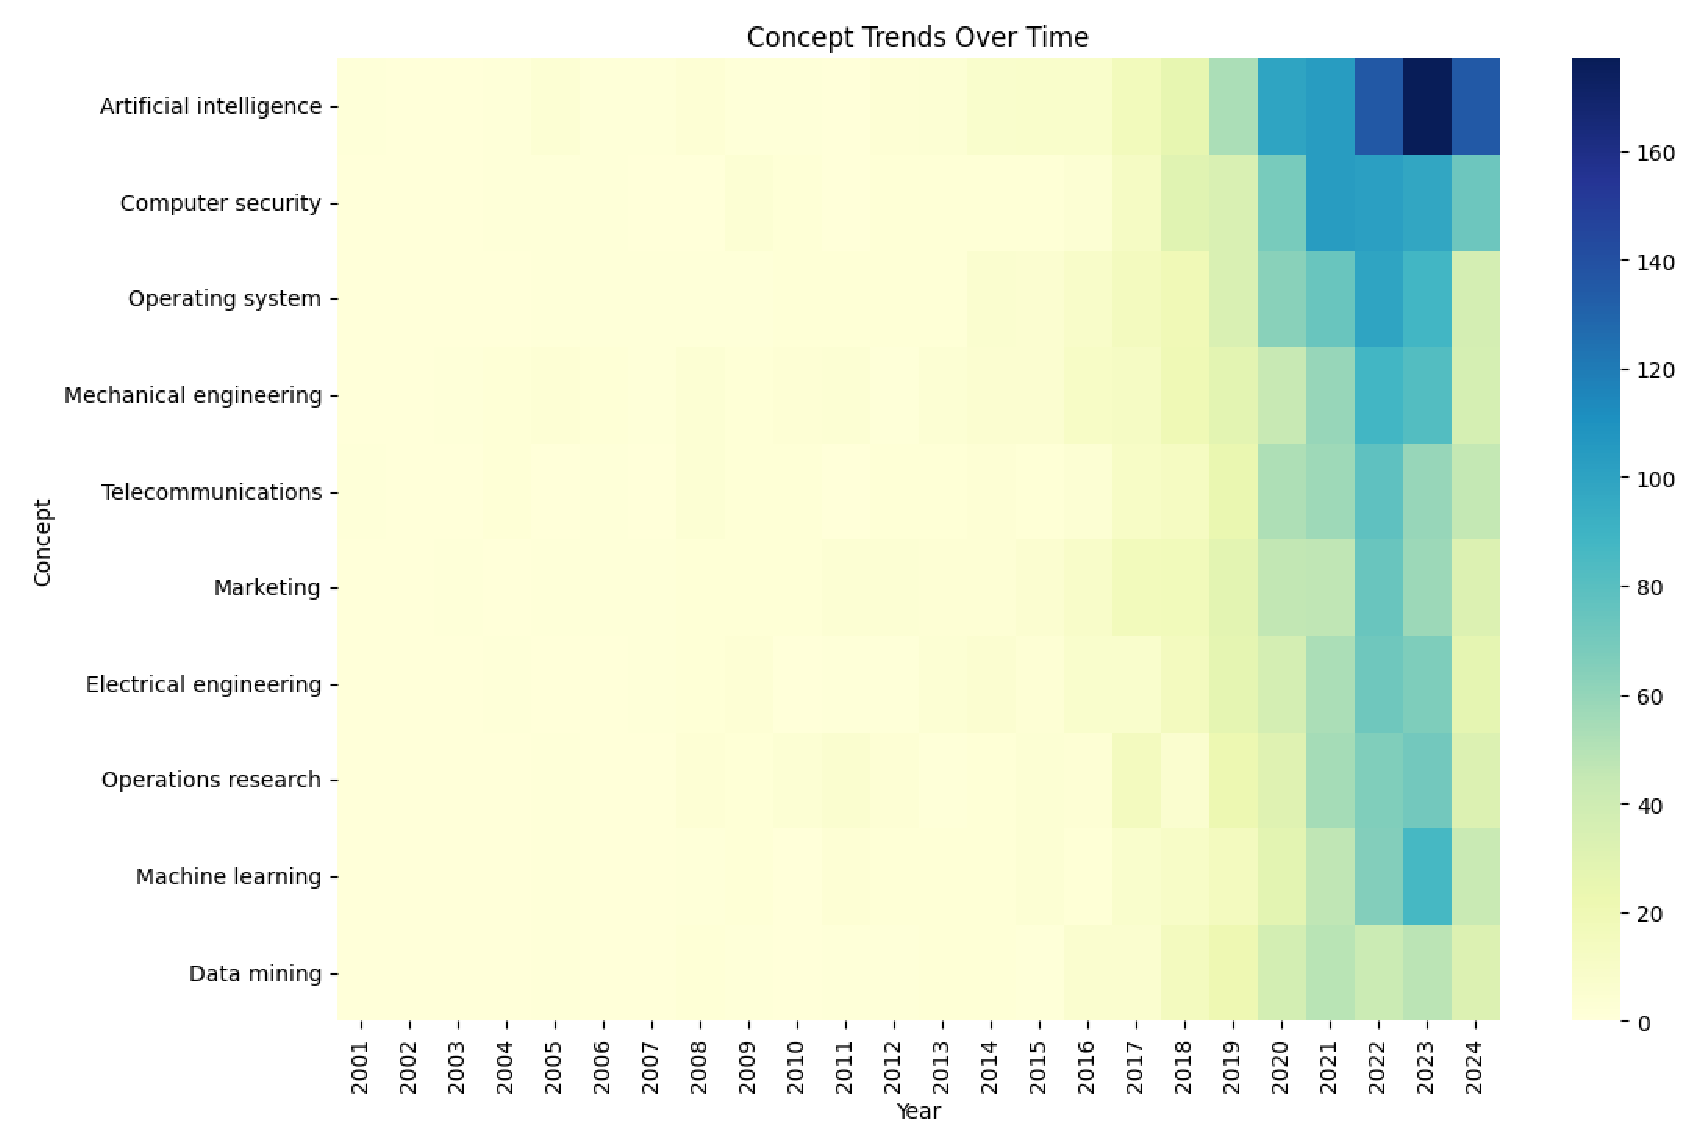
\includegraphics[scale=0.8]{pics/main_concept_trend_lowerlevels.eps}
		\caption{Detail-level OpenAlex concept distribution over time for the 10 most relevant terms}\label{fig:fig14}
	\end{figure}
	
	\section{Discussion}
	
	\section{Conclusion}
	Summarize key findings and future work.
	
	\bibliographystyle{elsarticle-harv}
	\bibliography{dxshippingbibliography}
	
\end{document}  % End of document